\documentclass[11pt,a4paper,oneside]{book}
\usepackage[hmargin={1.25in,1.25in},vmargin={1.25in,1.25in}]{geometry}
\usepackage{url}
\usepackage[utf8x]{inputenc}
\usepackage[T1]{fontenc}
\usepackage[english]{babel}
\usepackage{graphicx}
\usepackage{caption}
\usepackage{amssymb}
\usepackage{subcaption}
\usepackage{rotating}
\usepackage{multirow}
\usepackage{adjustbox}
\usepackage{listings}
\usepackage{hyperref}
\usepackage{fancybox}
\usepackage{enumerate}
\usepackage{amsmath}
\usepackage{indentfirst}
\usepackage[inline]{enumitem}
\usepackage{xcolor}
\usepackage{tikz}
\linespread{1.5}
\lstset{ %
  language=R,                     % the language of the code
  basicstyle=\footnotesize,       % the size of the fonts that are used for the code
  numbers=left,                   % where to put the line-numbers
  numberstyle=\tiny\color{gray},  % the style that is used for the line-numbers
  stepnumber=1,                   % the step between two line-numbers. If it's 1, each line
                                  % will be numbered
  numbersep=5pt,                  % how far the line-numbers are from the code
  backgroundcolor=\color{white},  % choose the background color. You must add \usepackage{color}
  showspaces=false,               % show spaces adding particular underscores
  showstringspaces=false,         % underline spaces within strings
  showtabs=false,                 % show tabs within strings adding particular underscores
  frame=single,                   % adds a frame around the code
  rulecolor=\color{black},        % if not set, the frame-color may be changed on line-breaks within not-black text (e.g. commens (green here))
  tabsize=2,                      % sets default tabsize to 2 spaces
  captionpos=b,                   % sets the caption-position to bottom
  breaklines=true,                % sets automatic line breaking
  breakatwhitespace=false,        % sets if automatic breaks should only happen at whitespace
  title=\lstname,                 % show the filename of files included with \lstinputlisting;
                                  % also try caption instead of title
  keywordstyle=\color{blue},      % keyword style
  otherkeywords={},
  commentstyle=\color{green},     % comment style
  stringstyle=\color{purple},     % string literal style
  escapeinside={\%*}{*)},         % if you want to add a comment within your code
  morekeywords={*, svmForecast, ly, getTestDf, renderPlotly, output, predPlot},            % if you want to add more keywords to the set
  deletekeywords={df, date, mode, window, gamma, rownames}
} 


\newenvironment{myitemize}
{ \begin{itemize}
    \setlength\itemsep{0pt}}
{ \end{itemize}                  } 


\makeatletter
\newcommand{\inlineitem}[1][]{%
\ifnum\enit@type=\tw@
    {\descriptionlabel{#1}}
  \hspace{\labelsep}
\else
  \ifnum\enit@type=\z@
       \refstepcounter{\@listctr}\fi
    \&\ \@itemlabel\ 
\fi}
\makeatother

\begin{document}
\nocite{*}

\begin{titlepage}
\begin{center}
\textbf{\textsc{UNIVERSIT\'E LIBRE DE BRUXELLES}}\\
\textbf{\textsc{Faculté des Sciences}}\\
\textbf{\textsc{Département d'Informatique}}
\vfill{}\vfill{}

\begin{center}{\Huge Machine learning approach for multi-step-ahead financial time series forecasting}\end{center}{\Huge \par}
\begin{center}{\large Jérôme Bastogne}\end{center}{\Huge \par}
\vfill{}\vfill{}

\includegraphics[keepaspectratio=true,scale=0.9]{img/ulbBlack.pdf}
\vfill{}\vfill{}
\begin{flushright}{\large \textbf{Promoteur :}}\hfill{}{\large Mémoire présenté en vue de}\\
{\large Prof. Gianluca Bontempi}\hfill{}{\large l'obtention du grade de}\\
{\large Ir. Jacopo De Stefani}\hfill{}{\large Licencié en Informatique}\end{flushright}{\large\par}
\enlargethispage{1cm}
\textbf{Année académique 2016~-~2017}
\end{center}
\end{titlepage}


\chapter*{Acknowledgements}


\tableofcontents


\chapter*{Abstract}


\chapter{Introduction}


Financial time series analysis drew significant attention in recent years. Traders, investors, markets analysts, anyone following the stock market is interested in a better understanding of price fluctuations. With all the medias and high-tech information constantly available, the stock prices can radically change from a day to another. The risks associated to falling prices are real and traders have to cope with them daily. A better understanding of stock prices behaviour would help traders to make decisions. This explains the consequent interest increase in accurate forecasting of future fluctuations.

The forecasting domain has largely been covered by linear statistical methods such as : ARIMA, GARCH... \cite{Holan} However, financial time series are often nonlinear and those methods are not able to capture the non-linearity of the financial time series. Some nonlinear methods have been studied, but they haven't been analysed as deeply as the linear ones described before \cite{BenTaieb}. Furthermore, generally in order to work, statistical methods requires that the data meet some assumptions, such as requiring stationary series,... On the other hand, machine learning aims to find patterns in data reducing the amount of assumptions on the process underlying the data.

Machine learning might therefore be more adequate to the forecasting of those series \cite{citeulike:13778368}. Machine learning is booming and yet has proven to be high performing. Also, the huge increase of the available data makes it too large for traditional analytics. Therefore machine learning is a more suitable choice.

Multi-step ahead forecasting strategies used in the context of this thesis have been largely inspired by the studies of \textit{Souhaib Ben Taieb} \cite{BenTaieb}. However, the performance of support vector machines for financial time series forecasting has not yet been studied for multi-step ahead forecasting. Therefore this will be one of my main contributions.

The aim of my work is twofold. On one hand I will focus on using machine learning techniques to forecast the future of financial time series. In particular, my goal is to compare the support vector machine algorithm's performance to more established algorithms for financial time series. 

Financial time series are known to be highly volatile. Volatility represents a measure of risk that investors have to cope with daily. Reacting defensively to a future risk increase requires some time to take actions and has to be done multiple days ahead. This reports the importance of multi-step ahead forecasting.  This study will cover the analysis of the volatility of financial time series.

On the other hand, the second objective is the development of a visual analysis tool to perform and compare multiple machine learning algorithms on financial times series. All the techniques described in the methodology section will be put into a tool that can be used without any prior knowledge about machine learning. The tool will run online in an autonomous way and its data will be updated continually and automatically. The purpose of the tool is to offer a visual, fast, up-to-date and configurable way to compare forecasting algorithms on financial time series such as $CAC40$, $S\&P 500$,...

One will find in this document an overview of the state of art concerning financial time series in chapter \ref{backgr}. First there will a quick reminder of fundamentals and basic definitions. After that, chapter \ref{methodo} will be dedicated to the methodology and the procedures to follow in order to achieve machine learning forecasting. Next will follow a presentation of the developed tool in chapter \ref{tool}. Finally, chapter \ref{results} will be devoted to experiences measuring the machine learning algorithm's performances and discussions on their results.




\chapter{Background} \label{backgr}

In this chapter, I'll review the basics of the prediction of time series in order to have a brief introduction to machine learning. Therefore this chapter will be a quick reminder of fundamentals alongside some formal basic definitions. 



\section{Efficient Market Hypothesis}

The efficient-market hypothesis (EMH) states that stock prices fully reflect all available information and that prices are immediately corrected by any news. This would mean that the market is unbeatable and therefore, forecasting would be impossible as the main assumption of forecasting is that any information of the past has some incidence on the future. Also some evidence argue against EMH proving that stock market is not efficient. Indeed it wrongly assumes that all investors are always rational. Also, sometimes only a few traders have knowledge of a particular new information jeopardising this theory. However, if this theory would hold, the best possible forecast would only be the use of the last observed value \cite{aamodt} : 

\begin{center}
    $Y_{n+1} = Y_{n}$
\end{center}


The question if the market is truly unbeatable still didn't reach any consensus. So while it is still only a theory, it is important to have an overview of the subject. \cite{emh}


\section{Definitions}


\subsection{Machine learning}

A very well known quote from \textit{Tom Mitchell} defines machine learning as : 

\vspace*{\fill} 
\begin{quote} 
\centering 
``A computer program is said to learn from experience E with respect to some class of tasks T and performance measure P if its performance at tasks in T, as measured by P, improves with experience E'' -- \textit{Tom Mitchell, Carnegie Mellon University}. 
\end{quote}
\vspace*{\fill}


Machine learning is helpful when there is a need of understanding a time series behaviour to make predictions on it, even if nothing is known about the nature of the time series. There exist different types of learning algorithms and some of them will be discussed in section \ref{MLalgs}.


\subsection{Time series}

A time series is a finite sequence of $n$ data points $Y_{t}$ $\epsilon$ $\Re$ observed over time. Points are often equally spaced by time intervals. All points are ordered by their timestamp and changing that order would change the meaning of the data. \cite{hyndman}

\subsubsection{Examples}

\begin{myitemize}
    \item Numbers of sales of a company each month of year 2016.
    \item Temperature measurements in a country over 20 years.
    \item Electricity consumption in Belgium measured every half-hour for 100 days, representing 144000 values.
    \item Unemployment rate in the United States (figure \ref{fig:US}).
\end{myitemize}

\begin{figure}[ht]
  \centering
    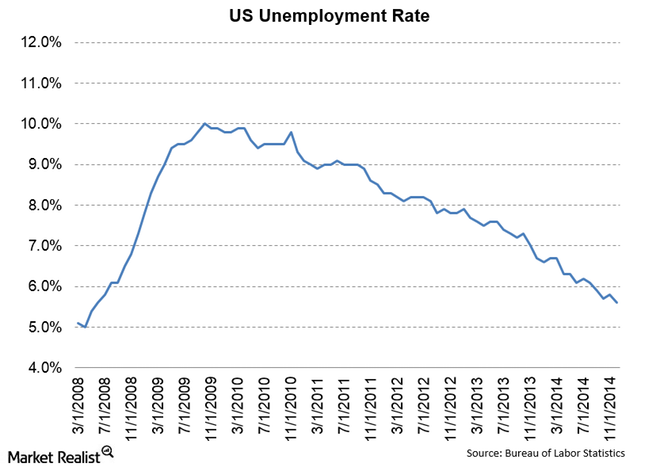
\includegraphics[scale=0.5]{img/Unemployment-Rate.png}
  \caption{Unemployment rate in the United States}
  \label{fig:US}
\end{figure}



\subsection{Forecasting}

One of the biggest interests of studying time series is forecasting. Indeed, based on the previous observations of a time series $Y_{1},...,Y_{n}$, could we predict the future observations  $Y_{n+1}, Y_{n+2},...$? 

It is possible under the strong assumption that a dependency between the past and the future exists. The challenge is to find the \textit{\textbf{model}} that describes the best the pattern of the time series.

Forecasts can be required for short-term, medium-term and long-term purposes. Short-term forecasting is about close in time scheduling and decision making, such as scheduling of tasks, personnel,... Medium-term forecasting helps to determine future resource requirements, such as hiring personnel, acquiring needed knowledge to handle particular tasks,... Finally, long-term forecasting is used for strategic planning with a long-term horizon. It is often a help to make long-term business decisions for a company. \cite{hyndman}


\section{Stationarity}

A (weak) stationary process is a process from which the mean, the variance and its covariance are constant over time; the distribution of $y_1$, $y_2$,... $y_n$ for each observation of a time series $y$ is independent of $n$. It is often a requirement for models that the time series has to be stationary. If it is not the case, some transformation can be applied to make it stationary. A time series can be made stationary by differencing, detrending or taking the logs or square roots of the time series. \cite{hyndman}



\section{Stochastic models}

Choosing a model is an important step in time series forecasting. A model's principal function is to describe how the most important \textit{\textbf{features}} of a time series can be combined to form a meaningful prediction. A \textit{\textbf{feature}} is an individual measurable characteristic, a variable. A model should explain how the past influenced the present and could be used to extrapolate the future. And if handling multiple time series, a model should explain how they affect each other. Finally, a model should accurately forecast future values of a time series. \cite{hyndman}

We will first have a look at traditional stochastic models, such as ARMA and ARCH, that were studied for a very long time. Later, we will compare them with some machine learning algorithms that, in comparison, are still booming.


\subsection{ARMA}

ARMA is the main statistical model for univariate linear time series forecasting. ARMA is a combination of auto regressive (AR[p]) and moving average (MA[q]) models. Auto regressive means that each value from the time series is regressed based on its previous values. Moving average means that the model uses previous forecast errors in a regression-like model. ARMA's general form is : 

\begin{equation}
Y_{t} = \sum\limits_{i=1}^p \phi_{i} Y_{t-i} +  \sum\limits_{i=1}^q \theta_{i} \epsilon_{t-i} + \epsilon_{t} 
\end{equation}

where $\phi_{i}$ and $\theta_{i}$ are the constant parameters and $\epsilon_{t}$ are independent errors also called \textit{\textbf{white noise}}. White noise is a sequence of uncorrelated components with a zero mean and a finite variance.

Regarding ARMA parameters : first, parameters $p$ and $q$ are estimated by looking respectively at the autocorrelation and partial autocorrelation functions. For the $AR(p)$ processes, the partial autocorrelation function becomes zero from lag $p + 1$. For the $MA(q)$ processes, the autocorrelation function becomes zero at lag $q + 1$. These are step of the so called \"Box–Jenkins model estimation\". \cite{boxjenk}

Then, parameters $\phi$ and $\theta$, respectively parameters of $AR$ and $MA$, can be estimated with various such as : Yule-Walker Estimation, Maximum Likelihood Estimation,...

However, the problem with ARMA is that it requires the time series to be stationary which isn't always the case. Otherwise, when the variance isn't constant, an ARCH model is the better choice. \cite{Holan}


\subsection{ARCH \& GARCH}

ARCH in an auto regressive (AR) conditional heteroscedastic (CH) model. Heteroscedastic means that the variance of a variable isn't constant over a determined interval of time. It is useful when studying financial time series because it illustrates the evolution of high variance changes for short periods of time, also described as volatility clustering. For example, if a market incurs a substantial drop, it can alert people to sell their stock before it drops even more. Therefore we can observe conditional periods of increased variance followed by calmer periods. \cite{Holan}

So, if we use ARCH as an auto regressive model of the variance of the series $y_t$ with zero mean, we can write the ARCH(q) model as : 
\begin{equation}\label{eq:arch}
\begin{matrix}
y_t = \sigma_t \epsilon_t \\
with \ \epsilon_t \sim iid(0,1) \\
\sigma_t^2 = Var(y_t \mid y_{t-1},..., y_{t-q}) = \alpha_0 + \alpha_1 y_{t-1}^2 + ... + \alpha_q y_{t-q}^2
\end{matrix}
\end{equation}


From there, GARCH (generalised ARCH) was introduced by adding moving-average components of the conditional variance to the ARCH model. The GARCH(p,q) model changes the definition of $\sigma_t^2$ in equation \ref{eq:arch} as : 

\begin{equation}
\sigma_t^2 = \alpha_0 + \sum_{j=1}^p\beta_j \sigma_{t-j}^2 + \sum_{k=1}^q\alpha_k y_{t-k}^2 
\end{equation}

where $ \beta_1,..., \beta_p \geq 0$ and $\alpha_1,...\alpha_q \geq 0$. Parameters $p$ and $q$ define the order of the model. \cite{Holan}





\section{Volatility}

Volatility defines the amplitude of variations of a time series. It is a key feature for financial time series analysis. Volatility represents a risk measure which is therefore directly related to risk management, a primary task of investors. Investors are vulnerable to time changing volatility that causes uncertainty in risk assessment. 

Volatility is a vague notion and an unobservable variable. It can be interpreted in multiple ways and therefore it has to be calculated with a proxy of conditional variance. It can either be seen as the standard deviation computed over a moving window of a determined size, it can be computed as the variance between returns, or it can be one of some of the definitions of volatility given by Garman and Klass \cite{garm} which will be described later in section \ref{vol}.

While GARCH models are known to be very well suited for volatility forecasting, I'll try to show through this thesis the capabilities of machine learning in that domain.

Note that volatility forecasting is directly linked with multi-step-ahead forecasting here. Indeed, knowing the risk degree only one day ahead is not enough for traders to react and take actions on the market. Having an idea of the behaviour of volatility several days in advance has a great added value for investors.




\chapter{Methodology}\label{methodo}

This chapter is dedicated to the \textit{modus operandi} of machine learning and forecasting. One can have an overall overview of the machine learning procedure on figure \ref{fig:ML}; the main \textit{\textbf{procedures}} are represented on the figure by black rectangles, and the blue ones represent what we have before the corresponding procedures, and what we get after each procedure. We will first have a look at the pre-processing phases. Then we will see the theory behind the models used in the tool. Finally, we will see how to choose a strategy with a model in order to make good predictions and how to quantify their performance.

\begin{figure}[ht]
  \centering
    \includegraphics[scale=0.55]{img/learningprocedure.png}
  \caption{Time series learning procedure to forecasting.}
  \label{fig:ML}
\end{figure}



\section{Pre-processing}

\subsection{Structure of the data}

One can choose to use the tool to forecast the original data as is, or can choose to forecast the continuously compounded returns or the volatility of the data instead.


\subsubsection{Prices (OHLC)}\label{OHLC}

When handling financial time series, a common dataset structure is a composition of : opening, high, low and closing prices (OHLC) and the volumes of the stock for each weekday. The OHLC format is very often used to view stock movements and provides more information for volatility calculations as explained in section \ref{volatility}. The low and high prices are the lowest and highest prices indices for a day and the opening and closing are respectively, the price at the start of the day when the stock market opens and the price when the stock market closes \cite{garm}. On figure \ref{fig:ohlc} we can see an example of OHLC chart of $CAC 40$ taken from $Yahoo!$ $Finance$ \cite{yahoo}. Each vertical bar represents the high and low for each day with on the left horizontal bar, the opening price, and on the right horizontal bar, the closing price. The bars are shown in green if the closing price is higher than the opening one, else red. 


\begin{figure}[ht]
  \centering
    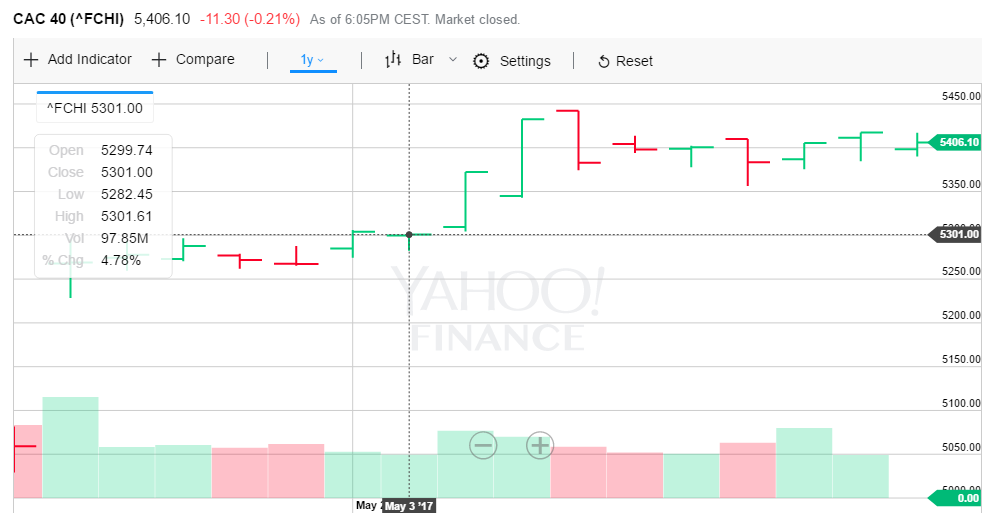
\includegraphics[scale=0.55]{img/ohlc.png}
  \caption{Open-high-low-close chart (OHLC).  \cite{yahoo}}
  \label{fig:ohlc}
\end{figure}


\subsubsection{Log returns}\label{logret}

Log returns are often more interesting for financial time series than the prices as is. Indeed, log returns gives us an unscaled values that are comparable with log returns of other time series. Log returns are defined as :

\begin{equation}
r_{t_i} = \ln\frac{P_{t_i}}{P_{t_{i-1}}}
\end{equation}

where $P_{t_i}$ defines the price at time $i$. 


\subsubsection{Volatility}\label{vol}

On the other side, volatility is the magnitude of changes in the prices of a financial asset. There are multiple ways of calculating the volatility of a financial time series, and one of the most suited should be one that considers historical OHLC prices (see \ref{OHLC}). The estimator of volatility used in this tool is one of the most practical and efficient based on a study from Garman and Klass \cite{garm}:

\begin{equation}\label{volatility}
\begin{matrix}
u = \ln\frac{P_t^{(h)}}{P_t^{(o)}} \qquad
d = \ln\frac{P_t^{(l)}}{P_t^{(o)}} \qquad
c = \ln\frac{P_t^{(c)}}{P_t^{(o)}} \\
\hat{\sigma}\left ( t \right ) = 0.511\left ( u - d \right )^2 - 0.019\left [ c\left (u + d\right ) - 2ud\right ] - 0.383c^2
\end{matrix}
\end{equation}

where $P_t^{(h)}$, $P_t^{(l)}$ and $P_t^{(c)}$ are respectively the high, low and opening prices at time $t$. The parameters $u$, $d$ and $c$ represent respectively the normalised high, low and close. The equation \ref{volatility} is a result of a multiple steps to reduce the bias and the variance. First, the authors tried do to take into account the nighttime volatilities by differencing the close and opening prices. After that, they used as another input the information contained in high and low prices. They finally came up to an optimisation problem that led to equation \ref{volatility}. \cite{garm}



\subsection{Normalisation}

Normalisation is often required by some algorithms to ensure convergence and it is also a stable way of comparing multiple models and algorithms. More importantly, it prevents a feature from dominating the others by being much larger. Therefore, before using any machine learning algorithm, the data is normalised as follows : 

\begin{equation}
{x}' = \frac{x - \mu }{\sigma }
\end{equation}

so that we have a normal dataset. Note that $\mu$, the mean of x, and $\sigma$, its standard deviation, both are calculated on the training set only with which the model will be trained. In this way, we avoid possible biases induced by not supposedly known information.




\section{Models}\label{MLalgs}

\subsection{Support vector machines}

\subsubsection{Definition}

Support vector machines (SVM) is a supervised learning model that performs classification by constructing an multi-dimensional hyperplane that optimally separates the data into two categories. SVMs can be used for regression by constructing an multi-dimensional hyperplane that minimises the cost function that measures the distance between the data points and the hyperplane.

SVM implements the structural risk minimisation principle which seeks to minimise an upper bound of the generalisation error rather than minimise the training error.

SVM uses linear models to implement nonlinear class boundaries through some nonlinear mapping of the input vectors into a higher dimensional feature space. A linear model constructed in the new space can represent a nonlinear decision boundary in the original space as seen on figure \ref{fig:svm}. In the new space, an optimal separating hyperplane is constructed. \cite{kim}\cite{liwang}\cite{Smola}


\begin{figure}[!h]
  \centering
    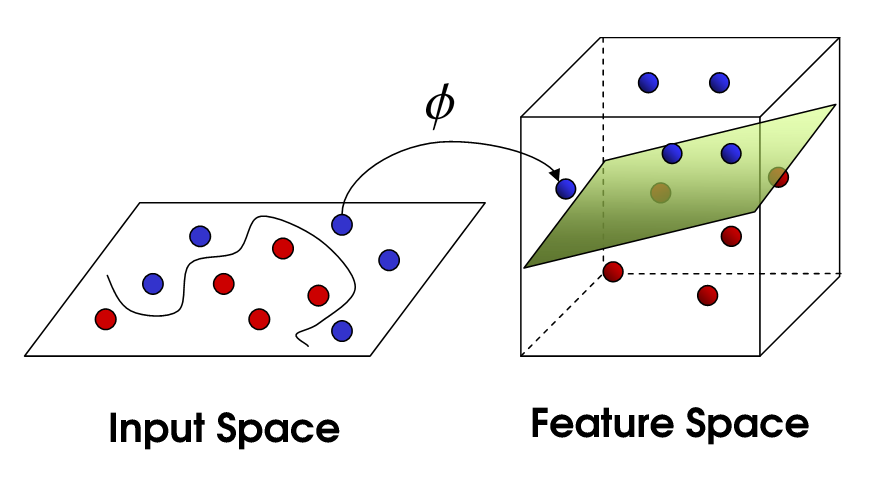
\includegraphics[scale=0.45]{img/svm.png}
  \caption{Transformation of the input space into a higher dimensional space with a kernel $\phi$ where the non-linearly separable data can be separated linearly by a hyperplane. \cite{svmpic}}
  \label{fig:svm}
\end{figure}


The support vectors are defined by the training examples that are closest to the maximum margin hyperplane and the support vector's number of coordinates are defined by the dimension space size. The margin of a training example is the distance of an example from the separating hyperplane. The maximum margin hyperplane gives the maximum separation between the decision classes as shown on figure \ref{fig:svm_linear_sep}. 

\begin{figure}[!h]
  \centering
    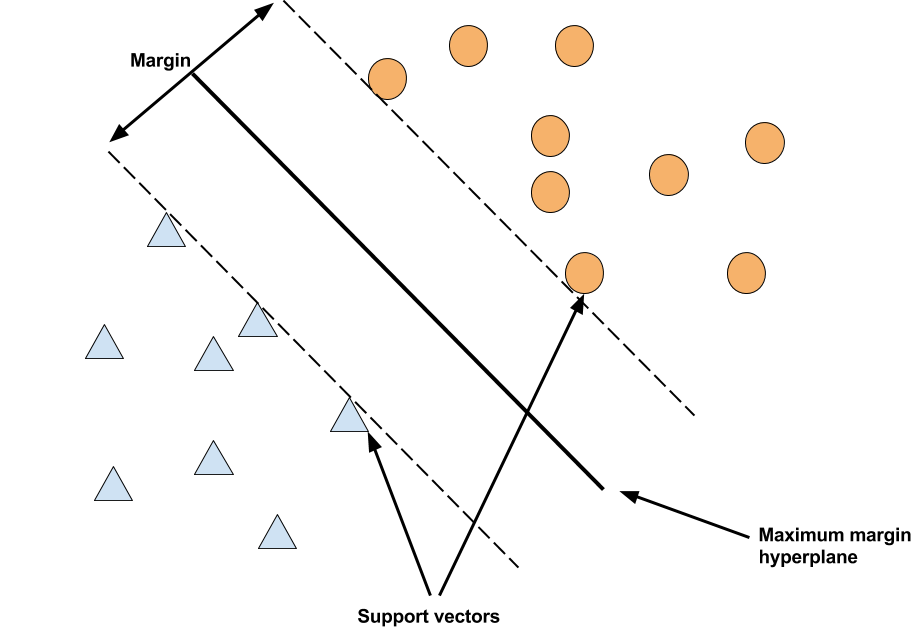
\includegraphics[scale=0.3]{img/svm1.png}
  \caption{SVM linearly separable case.}
  \label{fig:svm_linear_sep}
\end{figure}

Support vector machines can be applied to financial times series as a case of regression (SVR) by performing a linear regression in high dimensional feature spaces (instead of separating classes). They define the \textit{\textbf{loss function}} that ignores errors which are situated within the certain distance of the true value.

The transformation of a space into a higher dimensional space is done via a \textit{\textbf{Kernel}}. A kernel is a similarity function. Kernel functions have some tuning parameters. Overfitting can be avoided by allowing a small portion of the training data to lie outside the margin thanks to the slack parameter. For financial time series forecasting, a combination of kernels may be used as information can behave from different sources. This introduces the importance of choosing good parameters and the good combination of kernels (kernel selection). \cite{kim}\cite{liwang}\cite{Smola}


\subsubsection{Support vector regression theory}

Support vector machines will be detailed more in depth as it is the most novel algorithm and also the most promising. Therefore, this subsection will describe the most important mathematical steps to understand the intrinsic working of SVMs.

Given a training set $\left \{ \left ( x_{1}, y_{1} \right ), \left ( x_{2}, y_{2} \right ), ... \left ( x_{l}, y_{l} \right ) \right \}$ where $y_{i}$ is the output for the vector input $x_{i}$ and $x_{i} \in R^{n} , y_{i} \in R,  \forall i \in \left \{ 1,2, ...,l \right \}$, our goal is to find a function $f\left ( x \right )$ as flat as possible to make predictions different from at most $\varepsilon$ from those $y_{i}$ values for all the training data. This is called $\varepsilon$-SVM regression. $\varepsilon$-SVM makes that small deviations in the input still leave to the same output, making the method more robust. The $\varepsilon$-sensitive loss function that allows errors inside the $\varepsilon$ margin to be considered as zero is then given by :

\begin{equation}
L_{\varepsilon} = \left\{\begin{matrix}
0 \qquad\qquad\ \   if \ \left | y - f\left ( x \right )\right | \leq \varepsilon \\ 
\left | y - f\left ( x \right )\right | - \varepsilon \qquad otherwise
\end{matrix}\right.
\end{equation} \cite{Cortes}\cite{Smola} 

The empirical risk (training error) is given by the means of the errors :

\begin{equation}
R_{emp} = \frac{1}{n} \sum_{i=1}^n L_{\varepsilon}\left ( y_{i}, f\left ( x_{i} \right ) \right )
\end{equation}

Let's see how it works with the linear case where our function $f$ has the form :

\begin{equation}
f\left ( x \right ) = \left \langle w, x \right \rangle + b  \text{ with } w \in R^{n}, b \in R
\end{equation}

where $\left \langle ., . \right \rangle$ is the inner product.

To find a large-margin classifier, we want to minimise the norm of $w$. Therefore, by using regularisation our solution to the problem is :

\begin{equation}
\begin{matrix}
\min \frac{1}{2} \left \| w \right \|^{2}\\
\text{constrains:}
 \left |  y_{i} - (\left \langle w, x_{i} \right \rangle + b) \right | \leq \varepsilon 
 \end{matrix}
\end{equation}


\begin{figure}[!h]
  \centering
    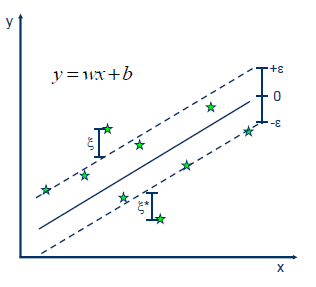
\includegraphics[scale=1]{img/SVR_2.png}
  \caption{Soft margin with the $\varepsilon$ bands and the $\xi$ slack variables. \cite{Sayad}}
  \label{fig:svr}
\end{figure}

We have to bear in mind the case where no such function $f\left ( x \right )$ satisfying the constraints for all points exists. So we have a problem when the optimisation problem is infeasible. Therefore, similarly to the "soft margin" loss function, we add positive slack variables $\xi_{i}\xi_{i}^{*}$ to allow some regressions errors (see figure \ref{fig:svr}). The principle is to separate the training set with a minimal number of errors. The addition of slack variables gives us a new formulation of the solution as :

\begin{equation}
\begin{matrix}
\min \frac{1}{2} \left \| w \right \|^{2} + C\sum_{i=1}^{l}(\xi_{i}+\xi_{i}^*)\\
\text{constrains :}
\left\{\begin{matrix}
y_{i} - (\left \langle w, x_{i} \right \rangle + b)\leq \varepsilon + \xi_{i}\\ 
-(y_{i} - (\left \langle w, x_{i} \right \rangle + b))\leq \varepsilon + \xi_{i}^*\\ 
\xi_{i} \geq 0\\ 
\xi_{i}^*\geq 0
\end{matrix}\right. 
\end{matrix}
\end{equation}


$C$\label{cost} is the constant parameter that represents the trade-off between the complexity of the model (i.e. the flatness of $f\left ( x \right )$, regularisation) and the number of regression errors (i.e. values outside the $\varepsilon$ margin, empirical risk). $C$ is called the regularised constant and takes care of avoiding overfitting. The higher $C$ is, the more we approach a hard-margin function and the less we will have misclassified individuals (overfitting).


By introducing Lagrange multipliers $\alpha_i \geq 0$, $\alpha_i^*\geq 0$ for each observation $x_i$, we can transform  $f\left ( x \right )$ and access its dual form which is easier to solve, but also it will help us for the nonlinear cases \cite{Cortes}\cite{Smola} : 


\begin{equation}
\begin{matrix}
\max -\frac{1}{2} \sum_{i,j = 1}^l \left ( \alpha _i - \alpha _i^* \right )\left \langle x_i, x_j \right \rangle - \varepsilon\sum_{i=1}^l\left ( \alpha _i + \alpha _i^* \right ) + \sum_{i=1}^l y_i\left ( \alpha _i - \alpha _i^* \right )\\
\text{constrains :}
\sum_{i=1}^l \left ( \alpha _i - \alpha _i^* \right) = 0 \\
0 \leq \alpha _i \leq C \\
0 \leq \alpha _i^* \leq C
\end{matrix}
\end{equation}


This equation can be solved by Sequential Minimal Optimisation and the solution to the regression problem is finally given by \cite{Cortes}\cite{Smola}:

\begin{equation}
f\left ( x \right ) = \sum_{i=1}^l \left ( \alpha_i - \alpha_i^* \right )\left \langle x_i, x \right \rangle + b
\end{equation}



For the nonlinear case, we don't search for the flattest function in the input space but rather in the feature space. The usefulness of the kernel comes from the fact that we don't have to explicitly compute the mapping of the input vector into the feature space $\phi(x)$. Instead we compute the inner products between the images of all pairs of data in the feature space very efficiently, this is known as the "kernel trick". The solution to the regression becomes :


\begin{equation}
f\left ( x \right ) = \sum_{i=1}^l \left ( \alpha_i - \alpha_i^* \right )K\left ( x_i, x \right ) + b
\end{equation}

where $K\left ( x_i, x \right )$ is the kernel function. The most popular kernel is named the Gaussian radial basis function kernel. The Gaussian RBF makes it the default kernel to use with no prior knowledge on the data and it is defined as : 

\begin{equation}
K\left ( x_i, x \right ) = \exp \left ( -\gamma \left \| x - x_i \right \|^2 \right )
\end{equation}

where $\gamma$\label{gamma} is the parameter that defines how far the influence a single training example is. It might be considered as a regularisation parameter. With a high gamma, the closest training examples from the decision boundary pull a lot more weight than farthest ones. On the other side, a small gamma means that the influence of $x_i$ is more important (and so imply large variance, small bias) and vice versa.

As a final note, one should keep in mind that he can combine multiple kernels in order to better capture the feature's natures, especially if the input is made of different sources.


\subsection{K-Nearest Neighbors}

KNN is a local nonlinear classification model that can also be used for regression. KNNs are often referred to as one of the simplest of all machine learning algorithms. Its principle is to find in the training set the input that is the most similar because similar input would have similar outputs. Note that here the input is a vector of points, and the size of the vector is the order of the model. 

Similarity between inputs can be computed with any distance function such as the Euclidean distance ($\sqrt{\sum_i \left (  x_i - y_i \right )^{2}}$). The KNN model output is then given by the mean of the k-nearest neighbors output as follows :


\begin{equation}
f\left ( x \right ) = \frac{1}{k}\sum_{x' \in KNN(x) } f\left ( x' \right )
\end{equation}

where $KNN(x)$ is the set of the k-nearest neighbors of $x$. There also exists a softer version of the k-nearest neighbors algorithm where instead of computing a mean, we compute a weighted average of each neighbor proportionally to their distance, the closer, the higher the weight is. The parameter k defines the bias-variance trade-off of the algorithm. The higher k is, the more samples we take from our training set, the lower the variance and the higher the bias are. In the other case, a small k will lead to overfitting. \cite{navot}



\subsection{Naive model}

Naive models can be computed in multiple ways. They generally are very simple and try to forecast the future as a mean of the past or a repetition of the last known value. In my case, I decided to implement the naive model by computing and repeating for each horizon, the mean of the last thirty values, i.e.\ a month more or less. So my naive model is defined as : 

\begin{equation}
\hat{y}_t = \frac{1}{k} \sum_{i=0}^{k} y_{t-1-i}
\end{equation}

where k is fixed to the number of days in a month.


\section{Forecasting strategies}\label{strat}

Once we have a prediction model, we need a strategy in order to compute the actual predictions. If the model is our ``regression function'', then the strategy is how to apply it to the time series for forecasting. Predictions can be done in two ways :

\begin{myitemize}
    \item One-step-ahead prediction.
    \item Multi-step-ahead prediction.
\end{myitemize}

Supervised learning approaches cover with success one-step-ahead prediction, which is the ability to predict the very next unknown value. However, multi-step-ahead prediction remains quite challenging.  k-step-ahead prediction is the prediction of the next $k$ unknown values of the time series. The challenges are to maintain low variance and low bias. Most often, strategies offer either one or the other. Figure \ref{fig:biasvariance} pictures the bias-variance trade-off that forecasting strategies have to cope with.


\begin{figure}[!h]
  \centering
    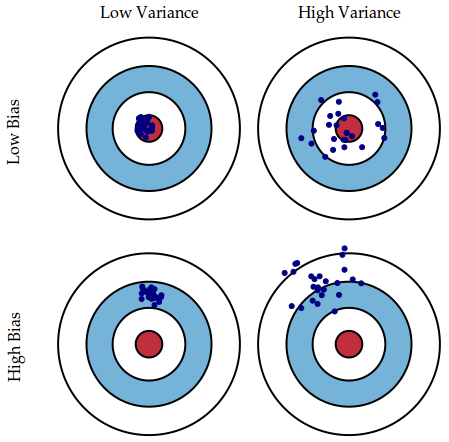
\includegraphics[scale=0.5]{img/bias-variance.png}
  \caption{Fundamental bias-variance trade-off of forecasting strategies. \cite{biaisvar}}
  \label{fig:biasvariance}
\end{figure}


\subsection{Multi-step-ahead strategies}

There exists some strategies for k-step-ahead prediction in the literature which the most common are described in the following section. \cite{Bonte}\cite{taiebonte}

\subsubsection{Recursive Strategy}

Also called iterated approaches, we iterate $k$ times with a one-step-ahead predictor. The one-step-ahead model $f$ to predict $y$ at time $t+1$ is first trained as : 

\begin{equation}
    y_{t + 1} =f(y_t,...,y_{t − e + 1}) + \epsilon_{t + 1}
\end{equation}

$\vee t \in \left[e,..., N - 1\right]$, where $N$ is the size of the time series and where $e$ is the order of the model as described in section \ref{embeddings}. \cite{souahib2}

Each time a value $y_{t+1}$ is predicted, it is used as input for the next iteration and therefore, errors propagate consequently. Recursive strategies can therefore be consequently biased. \cite{BenTaieb}


\subsubsection{Direct Strategy}

We make $k$ direct separate predictions $y_{t+h}$ $\vee h \in \left[1, k\right]$ for the next $k$ unknown values, a different forecasting model being used for each horizon. Individually, $k$ separate models are trained $\vee h \in \left[1, k\right]$ : 

\begin{equation}
    y_{t + h} = f_h(y_t,...,y_{t − e + 1}) + \epsilon_{t + h}
\end{equation}

$\vee t \in \left[e,..., N - k\right]$, where $N$ is the size of the time series. \cite{souahib2}

Though, direct approaches makes a conditional independence assumption which may be incorrect to do. It also needs bigger time series than the iterated approach because of iterated generative's nature. Direct strategies have then less inputs in comparison. This leads to high variance for little time series or large horizon forecasting. \cite{BenTaieb}


\subsubsection{MIMO (multi-input multi-output) Strategy}

The multi-input multi-output regression model returns a vector of $k$ consecutive predictions $\left\{y_{t+1},..., y_{t+k}\right\}$ in one step. One multi-output model $f$ is trained as :

\begin{equation}
    \left[y_{t + k},..., y_{t + 1}\right] = f(y_t,...,y_{t − e + 1}) + w
\end{equation}

$\vee t \in \left[e,..., N - k\right]$ and where $f : \mathbb{R}^d \rightarrow \mathbb{R}^k$ is a vector-valued function and $w \in \mathbb{R}^k$ is a noise vector. \cite{souahib2}

MIMO mimics the direct approach strategy but preserving the stochastic dependency of the time series. The problem involved with MIMO is that in order to keep that stochastic dependency, all horizons have to be forecasted with the same model structure which can be restrictive. \cite{Bonte}\cite{taiebonte}
    
    
\subsubsection{Rectify Strategy}

Rectify is a strategy that takes advantage of the strengths of both recursive and direct strategies. The principle is to first produce the predictions with the recursive strategy with a linear base model. As aforementioned, the results will be biased. Therefore, the second step of the strategy is to rectify the errors by adjusting the predictions with a nonlinear model with the direct strategy. This is supposed to reduce the bias of recursive linear systems. Rectify also proves to decrease variance's forecasts. \cite{BenTaieb}




\subsubsection{Dataset embeddings for multi-step forecasting}\label{embeddings}

The strategies described in this section above require the data to be held into a certain data structure. The structures will be described for the strategies used in the tool : the recursive and direct ones. 

Indeed, we want the model to learn how to predict a value $Y$ at time $t$ according to a number $e$ of past values, so we need to train a model that is able to predict $Y_t$ according to its $e$ past values. The number of $e$ past values, called the order of the model, is fixed beforehand.  

E.g.\ , for the recursive approach, if the order of the model is 4, our model will try to predict $Y_t$ according to  $Y_{t-1}, Y_{t-2}, Y_{t-3}, Y_{t-4}$. Therefore our model is trained by passing a structure as shown on figure \ref{fig:recursive} where each input is a vector of $e$ past values of each input $Y_t$ in the training set, where $e$ is the order of the model, and where the corresponding output is the value $Y_t$. 
 

\begin{figure}[!h]
\centering
\begin{minipage}{\textwidth}
\begin{minipage}{0.5\textwidth}
\begin{center}
\textbf{Recursive}
\begin{itemize}
\item A single model for every horizon $h$.
\item Forecast at step $h$ based on forecast at step $h-1$.
\end{itemize}
\vskip10pt
   \begin{footnotesize}
   \begin{tabular}{|cccc|c|}
   \hline
   \multicolumn{4}{|c|}{\textbf{input vector}} & \textbf{y} \\ \hline
   $y_{1}$ & $y_{2}$ & $y_{3}$ & $y_{4}$ & $y_{5}$\\ \hline
   $y_{2}$ & $y_{3}$ & $y_{4}$ & $y_{5}$ & $y_{6}$\\ \hline
   $...$ & $...$ & $...$ & $...$ & $...$\\ \hline
   $y_{t-4}$ & $y_{t-3}$ & $y_{t-2}$ & $y_{t-1}$ & $y_{t}$ \\ \hline
   \end{tabular}
   \end{footnotesize}
\end{center}
\end{minipage}
\begin{minipage}{0.5\textwidth}
\begin{center}
\textbf{Direct}
\begin{itemize}
\item A single model for each horizon $h$.
\item Forecast at $h$ step is made using $h^{\text{th}}$ model.
\end{itemize}
\vskip12pt
   \begin{footnotesize}
   \begin{tabular}{|cccc|c|}
   \hline
   \multicolumn{4}{|c|}{\textbf{input vector}} & \textbf{y} \\ \hline
   $y_{1}$ & $y_{2}$ & $y_{3}$ & $y_{4}$ & $y_{6}$ \\ \hline
   $y_{2}$ & $y_{3}$ & $y_{4}$ & $y_{5}$ & $y_{7}$ \\ \hline
   $...$ & $...$ & $...$ & $...$ & $...$ \\ \hline
   $y_{t-7}$ & $y_{t-6}$ & $y_{t-5}$ & $y_{t-4}$ & $y_{t-2}$ \\ \hline
   \end{tabular}
   \end{footnotesize}
\end{center}
\end{minipage}
\end{minipage}
\caption{Data structures required for the recursive and direct approaches.}
\label{fig:recursive}
\end{figure}


Therefore one additional step of the pre-processing is to embed the data into a similar structure than can be passed to a model according to the strategy used. Note that for the direct strategy, as explained, one model has to be built for each horizon $h$ and therefore, each model requires the data to be re structured into a similar matrix but with different offsets of $h$.



\section{Learning procedure}

Now that we have covered the theory on models and strategies, we can have a look at the different phases of the learning procedure as shown on figure \ref{fig:ML}.


\subsection{Model generation}

We want to find a function that gives us the closest values to the output depending on the input, output being the forecasted values that we want to fit to the test data and the input being our training data. That function is often called the hypothesis. \cite{BenTaieb}


\subsection{Parametric identification}

The parametric identification selects the parameters that minimises the disparity between the forecasted values and the output. Note that not all models have parametric identification. In the case of the SVM, we search for the values of the cost and gamma parameters (explained in section \ref{cost}) that reduce the most the gap between the forecasted values and the real output. For KNN, we have to find the number $k$ of instances that we take into account to determine similarities with classes. \cite{BenTaieb}


\subsection{Model validation}

The model validation phase is the process of examining the accuracy of the model. Estimating the errors is important, and if the evaluation is not satisfying enough, one should take the learning process back to model generation. A good way of measuring the performance of a model is by proceeding with a rolling window. Indeed, I chose a validation with a rolling window instead of a classical cross-validation because it ignores the temporal dependencies of time series. \cite{BenTaieb}


\subsubsection{Rolling window forecasts}\label{rwindow}


Rather than checking the performance of a model at one point in time, we would like to have a idea of how the model will generally perform. Sometimes we will have very accurate results, and other times the results will be worse, but we would like to have an idea of its general performance.

The principle is to use the model through the whole time series with a rolling window of a fixed size as shown on figure \ref{fig:rolling}. For each window, the data is separated into a training and a testing set. The model is then trained and predictions are made. By comparing those with the actual values in the testing set, we can compute errors and by averaging those over the whole time series we computed an averaged error. In the end, we get an average of errors that will be our performance indicator.

In the web tool I designed, the minimum size of the window is taken as two-thirds of the dataset and the window is offset by the same value as the horizon.


\begin{figure}[!h]
  \centering
    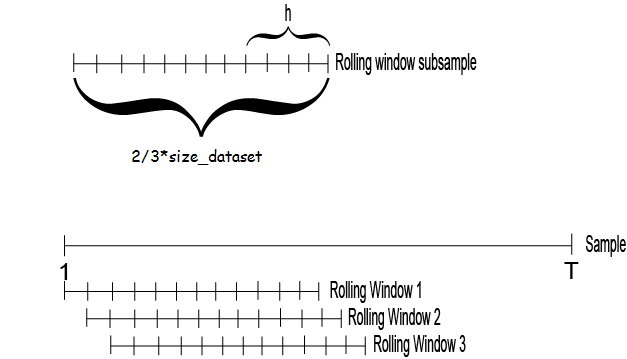
\includegraphics[scale=0.7]{img/rollingwindow.png}
  \caption{Rolling window principle\cite{rolling}.}
  \label{fig:rolling}
\end{figure}


\subsubsection{Error measures and forecasting performance evaluation}\label{errors}

This subsection will contain a brief description of all the errors measures that I show in my tool. I offer a large panel of choice regarding errors so that anyone can analyse the one that best suits its needs. 

The errors shown in the tool are listed in the table below  : \\


\begin{tabular}{|l|c|r|}
  \hline
   Full Name & Acronym & Formula \\
  \hline
  Mean Squared Error & MSE & $\frac{1}{n}\sum_{t=0}^n (y_t - \hat{y}_t)^2$ \\
  Root Mean Squared Error & RMSE & $\sqrt{\frac{1}{n} \sum_{t=0}^n (y_t - \hat{y}_t)^2}$ \\
  Mean Absolute Error & MAE & $\frac{1}{n} \sum_{t=0}^n |y_t - \hat{y}_t|$ \\
  Mean Absolute Percentage Error & MAPE & $\frac{1}{n} \sum_{t=0}^n  \mid 100 \cdot \frac{y_t - \hat{y}_t}{y_t}\mid$ \\
  Scaled Mean Absolute Percentage Error & sMAPE & $\frac{100}{n} \sum_{t=0}^n \cdot \frac{\mid y_t - \hat{y}_t\mid}{\frac{y_t+\hat{y}_t}{2}}$ \\
  Mean Absolute Scaled Error & MASE & $\frac{1}{n}\sum_{t=1}^n \left( \frac{\left| y_t - \hat{y}_t \right|}{\frac{1}{n-1}\sum_{i=2}^n \left| y_t-y_{t-1} \right|}\right)$ \\
  Normalized Mean Squared Error & NMSE & $\frac{1}{n}\frac{\sum_{t=0}^{n} (y_t-\hat{y}_t)^2}{var(y_t)}$ \\
  Normalized Naive Mean Squared Error & NNMSE & $\frac{1}{n}\frac{\sum_{t=0}^{n} (y_t-\hat{y}_t)^2}{\sum_{t=0}^{n} (y_t-\hat{y}_{Naive,t})^2}$ \\
  \hline
\end{tabular}  
\begin{flushright}
    \cite{Hyndman06} 
    \cite{nmse}
\end{flushright}



Remarkable notes : 

\begin{itemize}
    \item MSE, RMSE and MAE are scale dependent errors.
    \item MAPE and sMAPE are scale independant errors.
    \item MASE, NMSE and NNMSE are relative errors.
    \item MAPE is generally used for reporting to outsiders, because it expresses an error in percentages that anyone can imagine and understand.
    \item MASE is often the best performing performance meter because it avoids most of the problems induced by other error measures such as : scale independence, symmetry,... 
    \item NNMSE is a relative error showing how a model is better performing than the naive method. 
\end{itemize}



\subsection{Model selection}

Finally, model selection is the problem of choosing which method to use for a pool of possible methods. The best model should be chosen as the final model with the best related parametrisations. What is described as the best model is the model that performs the best on the validation set (i.e.\ testing set). That model should have the strongest capability of generalising, a good balance between fitting rightness and simplicity. \cite{BenTaieb}





\chapter{Forecasting tool}\label{tool}

As a major contribution for my master's thesis, I developed a web application tool in \textbf{$R$} that offers an easy and fast way to compare different machine learning models, forecasting some financial time series. The tool runs online and allows anyone to choose a financial time series, modify it, apply some machine learning models on it and tuning their parameters. 

The rest of this chapter includes a tutorial on how to use the tool, information on the data sources and the algorithms used in this tool and a section on how to include more models and data sources. 


\section{Presentation of the tool}

This section describes how the tool works and what its components are. The web page is divided in three tabs : one for the data selection and visualisation, the second one to try and compare forecasting models and the last tab is for errors analysis. 

Let's have a look at the first tab on figure \ref{fig:tool1} and its components descriptions.

\subsection{Tab : Data inspection}


\begin{figure}[!h]
  \centering
    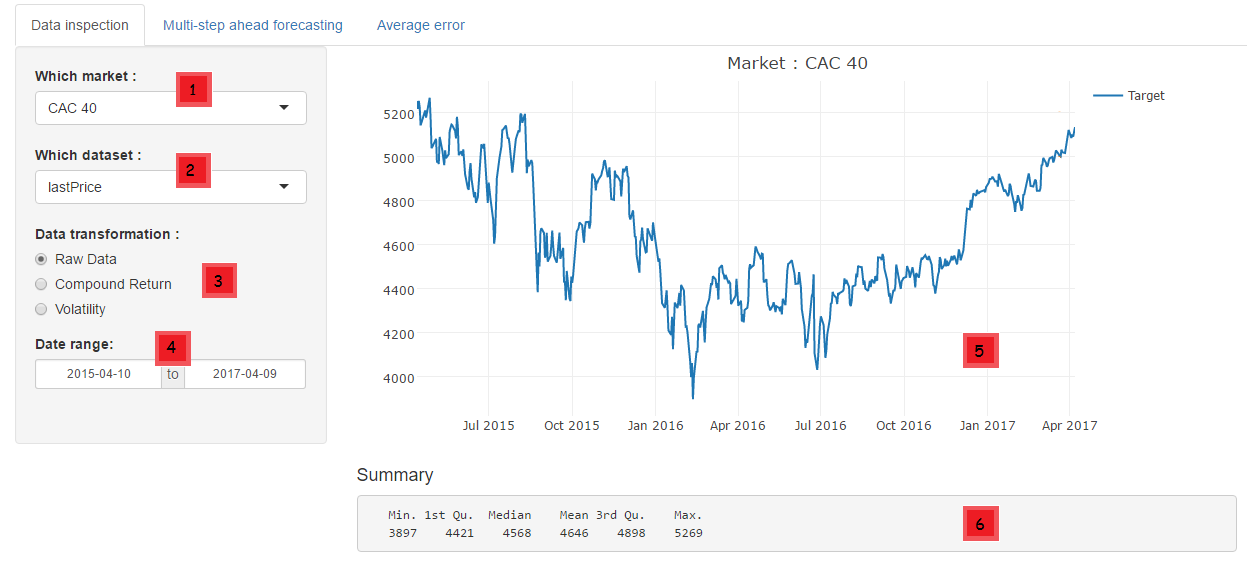
\includegraphics[scale=0.44]{img/tab1.png}
  \caption{View of the first tab of the tool.}
  \label{fig:tool1}
\end{figure}


\begin{enumerate}
\item This option allows one to choose a market. The corresponding data will be downloaded from $Yahoo!$ $Finance$ on its web link \url{http://finance.yahoo.com/} \cite{yahoo}. The download of the data is handled by the $quantmod$ package as explained in section \ref{libraries} and the nature of the data is explained in section \ref{datasets}. The data is automatically refreshed by the tool when new data is available.
\item For each market there are different selectable options such as : the opening, closing, high and low prices and the volume.
\item Rather than using the raw data, a transformation can be selected among the compound returns introduced in section \ref{logret} and the volatility of the data defined in section \ref{volatility}.
\item The time series can be cut in time as desired by adjusting the starting date on the left and the end date on the right. This way, one can position the time series himself wherever he wants back in time.
\item A plot to visualise the data belonging into the chosen date range and with the chosen transformation options.
\item A summary of the data showing basic informations like the mean, first and third quartiles,...
\end{enumerate}


\subsection{Tab : Multi-step ahead forecasting}

\begin{figure}[!h]
  \centering
    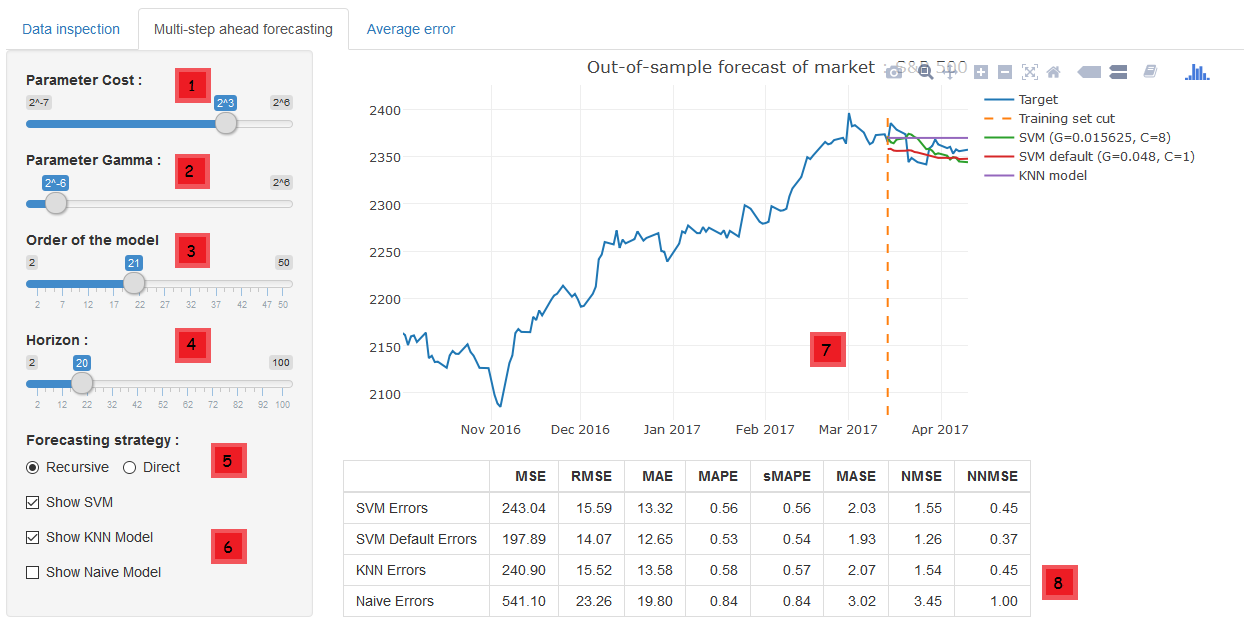
\includegraphics[scale=0.44]{img/tab2.png}
  \caption{View of the second tab of the tool.}
  \label{fig:tool2}
\end{figure}

\begin{enumerate}
\item\inlineitem Those are the configurable parameters of the SVM : C, the cost \ref{cost} and $\gamma$ \ref{gamma}, the Gaussian RBF kernel parameter. The Knn algorithm, from the $gbcode$ $R$ package\cite{gbcode}, already finds the best parameter for $K$ with a fast automated cross-validation.
\item This the order of the model discussed in section \ref{embeddings}, i.e.\ the number of days which are used to predict a value $Y_t$ at time $t$.
\item The horizon is the number of days we aim to predict in multi-step ahead forecasting.
\item The strategies are defined in detail in section \ref{strat}.
\item Those are some options to enable or disable the plotting of the models for a clearer visibility.
\item This is the resulting plot with its legend. The plot is made with the library \textbf{plotly} \cite{plotly} that gives a lot of options like zooming, downloading,... The orange dotted line shows the separation between the training set and the test set. Here, we are manually toying with parameters and therefore the line represents the horizon cut, which may be different during model validation.
\item This is a short table which resumes the errors of the models, as explained in section \ref{errors}, for the current forecasting. For a more general idea of how a model is usually performing, one should refer to the third and last tab of the web page. 
\end{enumerate}



\subsection{Tab : Average error}

\begin{figure}[!h]
  \centering
    \includegraphics[scale=0.44]{img/tab3.png}
  \caption{View of the third tab of the tool.}
  \label{fig:tool3}
\end{figure}


\begin{enumerate}
\item\inlineitem\inlineitem\inlineitem\inlineitem\inlineitem Those are the same parameters as those in the second tab.
\item This is a table of means of errors. Using the selected parameters, each model is applied through the whole dataset with a rolling window validation. The shown values are the averaged errors for each window as explained in section \ref{rwindow}.
\end{enumerate}



\section{Libraries}\label{libraries}

The tool is written in \textbf{$R$} \cite{R} and its web client-server part is mostly handled by a library called \textbf{Shiny} \cite{Shiny}.

\textbf{Shiny} is a library that proposes a web application framework that handles everything, including client-server, on itself. It allows one to only care about the functionalities of the code and the library will take care of how things are updated on the client part, how the client interacts with the server, ...

As for the rest, I use \textbf{Plotly} \cite{plotly} for the nice visual appearance plots and their nice interaction with the user. I use \textbf{e1071} \cite{e1071} for the SVM's models and \textbf{gbcode} \cite{gbcode} for the KNNs models.

Finally, the \textbf{quantmod} \cite{quantmod} package is a quantitative financial modelling framework and can be used for modelling in finance. The function $getSymbols$ of this library is used to download the datasets from the Internet.



\section{Datasets}\label{datasets}

The tool proposes some default datasets such as data from $CAC40$, $S\&P 500$,... These datasets are directly downloaded from $Yahoo!$ $Finance$ on its web link \url{http://finance.yahoo.com/} \cite{yahoo} and are daily refreshed. The data is publicly available and entirely free. 

Each dataset is composed of : dates, opening, high, low and closing prices (OHLC) and the volumes of the stock for each weekday. Data is available with a daily granularity and without any delay.


\section{Updates itself automatically}

The tool ensures that the data is automatically refreshed when new data is available. This is handled by the \textbf{Shiny} interface which is very reactive in its conception and acts in the same manner as the well known $Observer$ pattern. Indeed, \textbf{Shiny} gets notified when a reactive variables, i.e.\ $observable$ variables, are modified. The trick here is to invalidate the data set, which is a function that forces \textbf{Shiny} to react as if the data set was modified in order to trigger the update function. \textbf{Shiny} offers a built-in invalidation function associated with a timer that can be parametrised. When new data is downloaded, the models are also automatically updated with the new data without having to do anything. This is an important feature of the tool because it really shows its autonomy. The tool acts like a standalone app that constantly provides up-to-date information. 


\section{Code}

Due to the \textbf{Shiny} library, the code of the tool is very loosely coupled and easy to read. The code is decomposed in one file for each of the client-server parts, one configuration file, one for the errors measurements and one file per machine learning algorithm. 

There is no apparent links between the server and the client because \textbf{Shiny} handles it all. The client part contains a list of widgets to display accompanied by their positioning and a unique tag that refers to a variable from the server that they will be linked to. On the other side, the server contains all the logic of the program and stores its results in variables that the client will access thanks to their tag/variable name.

The configuration file, for its part, contains a list of datasets twinned with their respectively tag reference on $Yahoo!$ $Finance$. 

The rest of this section contains more information on how one could tweak the code and integrate new datasets and models.


\subsection{Add new datasets}

To add a new dataset, one has to find the tag reference of the market on $Yahoo!$ $Finance$ (can be found on \url{http://finance.yahoo.com/} \cite{yahoo}) and add it to the configuration file following the same pattern as those already added; see the content of the configuration file below : 


\begin{lstlisting}
markets        <- c( "^FCHI",  "^IXIC",   "^GSPC")
names(markets) <- c("CAC 40", "NASDAQ", "S&P 500")
\end{lstlisting}

where the $markets$ are the tags, and the $names(markets)$ are the names displayed in the application.


\subsection{Add new models}

To add a new model, one can make a new function that takes in input a dataframe, a horizon and more parameters, and that returns the final predictions as a list of values. As an example, below is the header of new dummy predictor that shows all the required functionalities a new model function should contain : \\


\begin{lstlisting}
modelNameForecast <- function(df, horizon, window, strategy, 
                                    parameter1, parameter2){
        # df is a dataframe
        # horizon and window are the multi-step-ahead parameters
        # strategy is either recursive or direct
        # the rest are specific model parameters
    ...
    return predictedY # the function returns a vector of predicted values
}
\end{lstlisting}


On the client part, nothing has to be changed. Instead, there must be some inclusions of the new model computations on the server part.

The server has then to be updated by adding the new model in the following functions : \textit{predPlot}, \textit{predTable}, \textit{errorTable}. They respectively correspond to the plotting function of the second tab, the predictions errors table on the second tab and the averaged errors of the rolling window table on the third tab of the tool. As an example, below is a piece of code of the function \textit{predPlot} : \\

\begin{lstlisting}
output$predPlot <- renderPlotly({
    # Initial plot
    p <- plot_ly(y = df$target, x = df$date, type = 'scatter',
                    mode = 'lines', name = 'Target')
    ...
    # Add forecasts for each model
    predictedY <- svmForecast(df, trainingcut(), window(), gamma(), 
                                    cost(), strategy())
    p <- p %>% add_trace(x = getTestDf()$date, y = predictedY, 
                                mode = 'lines')
    ...
}
\end{lstlisting}

First, the plot is created with \textbf{plotly}, and then the traces of each model's predictions are added to the plot. 

Another example is the function \textit{predTable} that shows the errors table on the second tab of the tool : \\

\begin{lstlisting}
output$predTable <- renderTable(rownames = TRUE, bordered = TRUE, {
    df <- getDf()
    ...
    
    # Get predictions for each model
    svmPredY <- svmForecast(df, trainingcut(), modelOrder(), gamma(), cost(), strategy())
    defaultSvmPredY <- svmForecast(df, trainingcut(), modelOrder(), strategy = strategy())
    knnPredY <- modelSelectionKNN(df$target, trainingcut(), modelOrder(), strategy())$forecasts
    naivePredY <- naiveForecast(df, trainingcut())

    ...
    
    # Show the means of all errors in table
    as.data.frame(getErrors(svmPredY, defaultSvmPredY, knnPredY, naivePredY, getTestDf()$target))
  })
\end{lstlisting}  
  
As one can see, the code is just about forecasting values with each model and compute the errors with the actual values. Adding a new model here is about adding a call to the model and adding the predictions to the errors computations. The function \textit{errorTable} is nearly the same.

A special note : the \textbf{Shiny} library handles the fact that if the same function is called for multiple outputs, it is only computed once and the same results are returned for each output. Therefore, we can call \textit{svmForecast} for the plotting and the errors computations without doing over-computations because internally, \textbf{Shiny} handles it all and will update the results automatically if any of the parameters is changed.

So any new model can be included in those functions by following the same structure as the models already present. Nothing else has to be changed.


\chapter{Results}\label{results}

In this chapter, one will find the descriptions of the experiments I conducted in order to identify the best parameters for each model, i.e.\ the parameters that lead to the smallest errors. After exploring experiments' results, one will find a section comparing and discussing the results of the algorithms between them.


\section{Description of my experiments}


I will conduct experiments to see which algorithms work best for the prediction task. I will grid search for the best parameters of each algorithm to perform forecasting. I will compare the averaged MSE, NMSE and MASE over a rolling window validation as explained in \ref{rwindow}. First I will run the experiments on a reduced history of 9 months in order to quickly select the most efficient model. After that, I will run the same experiments on a longer history of 10 years to evaluate the performance of the optimal models over the long term and see if there is a model that is consistently performing better than the others.

The experiments will be run on the volatility of the \textit{CAC40} times series. I will use two different proxies for the volatility : the proxy described by equation \ref{volatility} also used in the tool (proxy 1), and the rolling standard deviation with a window of 21 days (proxy 2). It will be interesting to see if the smoothness of proxy 2 has any positive effects for forecasting, or if daily volatility has more benefits. All the experiments will be run with a window of 21 days and a horizon of 7 days which are values that I found to perform well while using my tool.

I made preliminary analyses by testing the SVM parameters with the tool I developed in order to better lead my grid searches. Therefore, not all results will be displayed with the same granularity.

Concerning the search grid process of SVM parameters, searching through exponentially growing sequences, such as powers of 2, for $C$ and $\gamma$ is a practical method to identify good parameters. \cite{Hsu}

The structure of the rest of this chapter is divided as follows : first are shown the results for the reduced history before the longer one. For each history, the results are divided between first proxy 1, then proxy 2. Each proxy section shows first the results of the SVM search grid. Then will be displayed, for each error measure (MSE, NMSE, MASE), the results with the best parameters. Finally, a discussion of the results will end the chapter.



\section{Reduced history}

I first ran the experiment on a 9 months history. On figure \ref{fig:plot6m}, one can observe the plots of the time series with the applied proxies.


\begin{figure}[!h]
\centering
\makebox[\linewidth]{%
\begin{subfigure}{.55\linewidth}
  \centering
  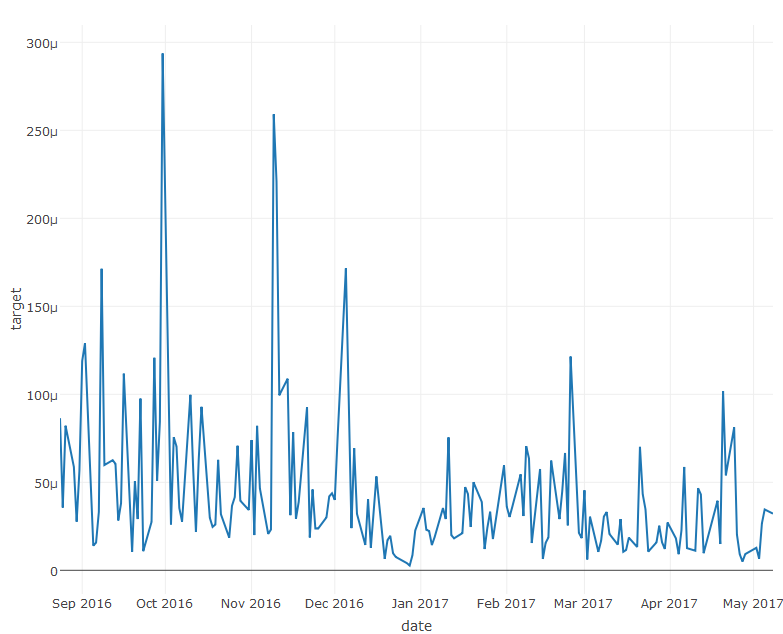
\includegraphics[width=\linewidth]{img/plot6sigma.png}
  \caption{Using proxy 1.}
  \label{fig:sub1}
\end{subfigure}%
\begin{subfigure}{.55\linewidth}
  \centering
  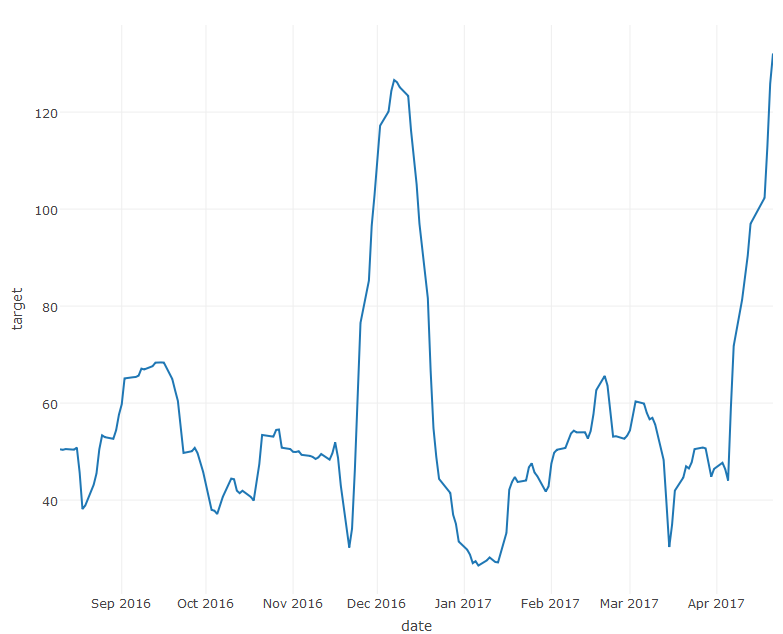
\includegraphics[width=\linewidth]{img/plot6ma.png}
  \caption{Using proxy 2.}
  \label{fig:sub2}
\end{subfigure}}
\caption{Plots of the reduced time series using the two proxies.}
\label{fig:plot6m}
\end{figure}


One will find in the rest of this section, first the results using proxy 1, then the results using proxy 2.

The results of the search grid for the SVM parameters can be visualised on the heat maps on figure \ref{fig:heat6mp1} for proxy 1, and \ref{fig:heat6mp2} for proxy 2, where the resulting errors are displayed according to the parameters. The complete numeric results of the search grids can be found in appendix \ref{6mapp}. On the heat maps, the abscissa shows the different values for $\gamma$ and the ordinate shows the different values for $C$, the cost. The scales are not the same for all heat maps, they are rather zoomed in the interesting zones. On the right of each heat map stands a vertical bar mapping colors with values in order to distinguish between error scales. The minimum errors colors are located on the bottom of the bar.

As on can see on the heat maps, the most optimal cost and gamma parameters seem to lie on a diagonal. This is an indication of how one should use those parameters.

Then, for each proxy, one will find the results of the experiments for SVM, KNN and the naive method regrouped for each error measure. First, the results will show a table of the parameters that lead to the smallest related error measure, which is the averaged error over the whole rolling window validation process. Below the table, one will find box-plots of all the errors for the best parameters. Bear in mind that outliers are not shown on the box-plots. With the help of those plots, one can better imagine the relevancy of the averaged errors.



\clearpage
\subsection{Proxy 1 results}
 \begin{center}
\begin{tabular}{|c|c|c|c|}
\hline
& \multicolumn{3}{|c|}{\textbf{Proxy 1}} \\ \cline{2-4}
& \textbf{MSE} & \textbf{NMSE} & \textbf{MASE}          \\ \hline
Cost  & $2$             &$2^9$      & $2^8$          \\ 
Gamma & $2^{-13}$       &$2^{-19}$  & $2^{-17}$ \\ 
Error & $5.443549e-10$  &$5.098590$ & $1.2278$     \\ 
\hline
\end{tabular}


 \begin{figure}[!h]
\centering
\makebox[\linewidth]{%
\begin{subfigure}{.55\linewidth}
  \centering
  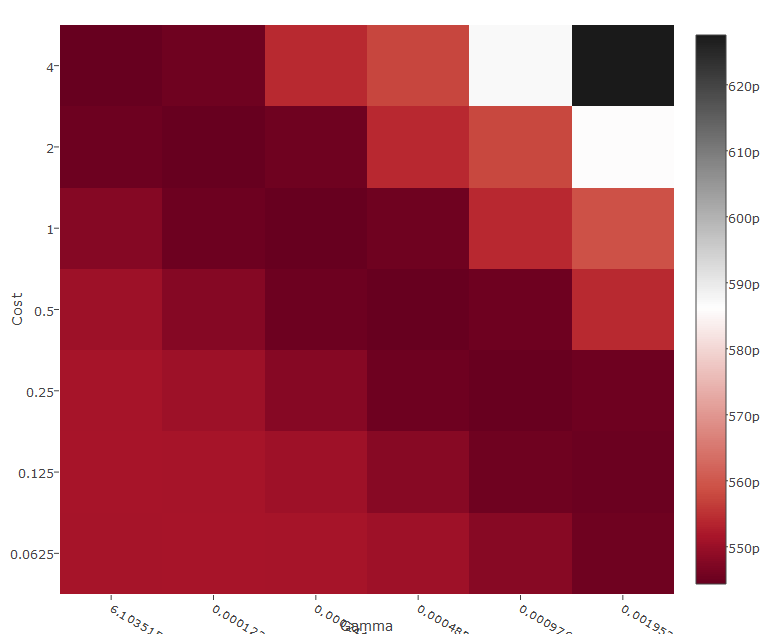
\includegraphics[width=\linewidth, height = 0.32\textheight]{img/6mMSEsigma.png}
  \caption{MSE using proxy 1.}
  \label{fig:heat1}
\end{subfigure}%
\begin{subfigure}{.55\linewidth}
  \centering
  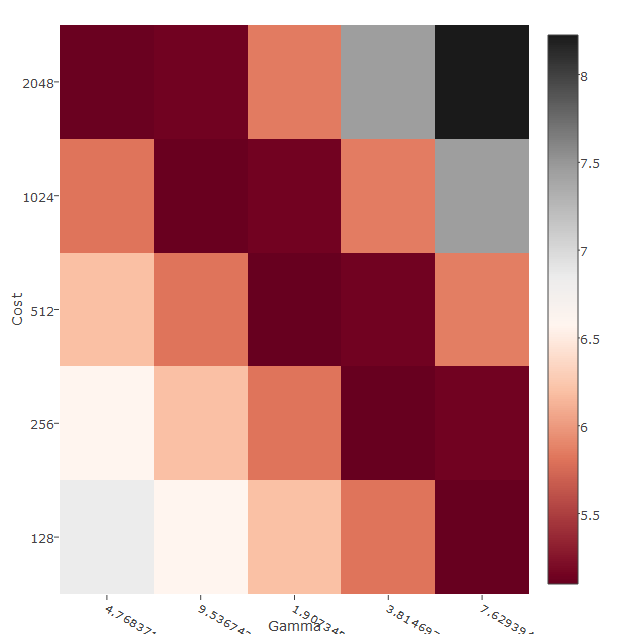
\includegraphics[width=\linewidth, height = 0.32\textheight]{img/6mNMSEsigma.png}
  \caption{NMSE using proxy 1.}
  \label{fig:heat2}
\end{subfigure}}
  \centering
  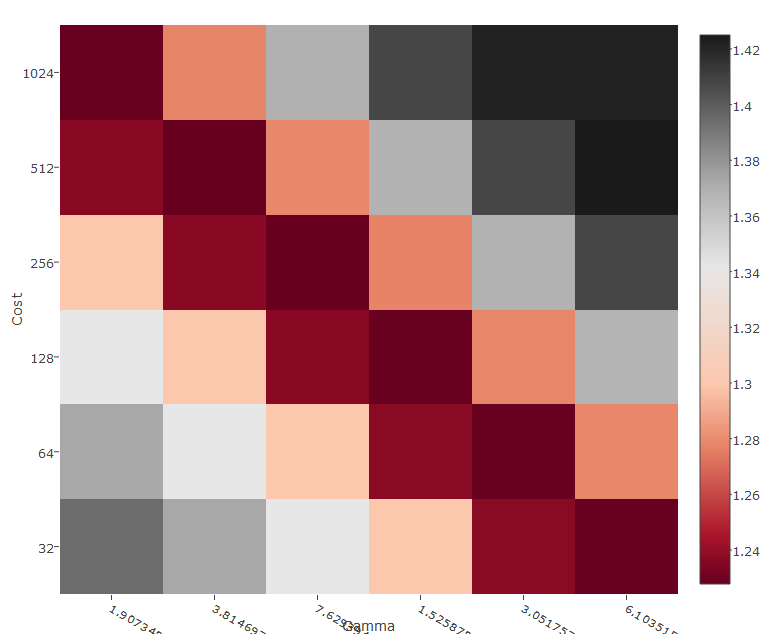
\includegraphics[width=0.6\linewidth, height = 0.34\textheight]{img/6mMASEsigma.png}
  \caption{MASE using proxy 1.}
  \label{fig:heat3}
\caption{Heat maps resulting of the SVM grid search for each error using proxy 1.}
\label{fig:heat6mp1}
\end{figure}\end{center}


\clearpage
\begin{figure}[!h]
\centering
\begin{tabular}{|c|c|c|}
   \hline
   & \multicolumn{2}{|c|}{\textbf{MSE}} \\ \cline{2-3}
   & \textbf{Errors} & \textbf{Parameters}          \\ \hline
   SVM  & $5.443549e-10$        & $C = 2$, $\gamma = 2^{-13}$          \\ 
   KNN & $6.492108e-10$ & $K = 15$ \\ 
   Naive & $6.144618e-10$ &      \\ 
   \hline
   \end{tabular}
\caption{Comparison of MSE errors with the best parameters configurations.}
\label{fig:table6mMSEp1}
\centering
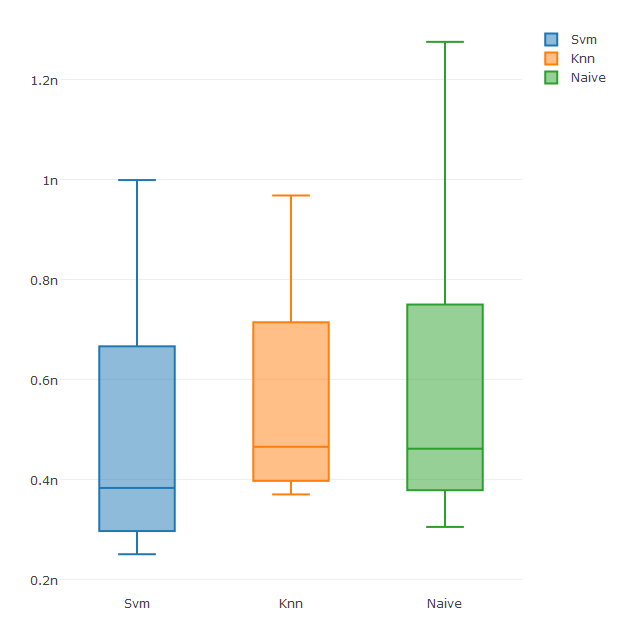
\includegraphics[width=\linewidth]{img/6mproxy1MSE.png}
\caption{Box plots of the MSE errors with the best parameters for the rolling window cross-validation with proxy 1. On the ordinates, $n$ represents $n := 10^{-9}$.}
\end{figure}


\begin{figure}[!h]
\centering
\begin{tabular}{|c|c|c|}
   \hline
   & \multicolumn{2}{|c|}{\textbf{NMSE}} \\ \cline{2-3}
   & \textbf{Errors} & \textbf{Parameters}          \\ \hline
   SVM  & $5.098590$        & $C = 2^9$, $\gamma = 2^{-19}$          \\ 
   KNN & $7.424236$ & $K = 15$ \\ 
   Naive & $7.059421$ &      \\ 
   \hline
   \end{tabular}
\caption{Comparison of NMSE errors with the best parameters configurations.}
\label{fig:table6mNMSEp1}
\centering
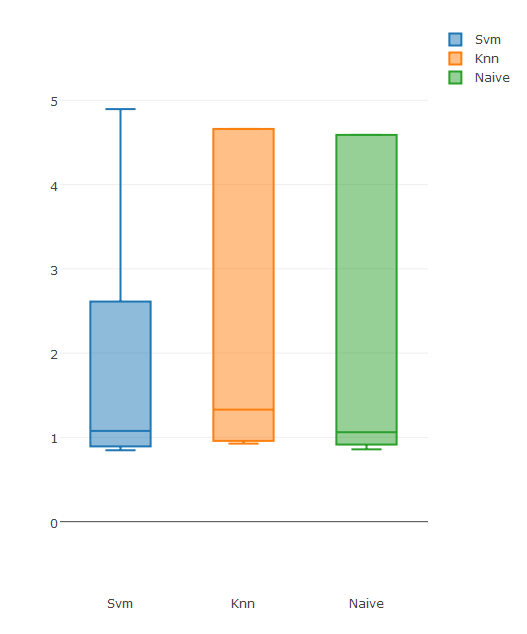
\includegraphics[width=\linewidth]{img/6mproxy1NMSE.png}
\caption{Box plots of the NMSE errors with the best parameters for the rolling window cross-validation with proxy 1.}
\end{figure}


\begin{figure}[!h]
\centering
\begin{tabular}{|c|c|c|}
   \hline
   & \multicolumn{2}{|c|}{\textbf{MASE}} \\ \cline{2-3}
   & \textbf{Errors} & \textbf{Parameters}          \\ \hline
   SVM  & $1.2278$        & $C = 2^8$, $\gamma = 2^{-17}$          \\ 
   KNN & $1.518099$ & $K = 15$ \\ 
   Naive & $1.483807$ &      \\ 
   \hline
   \end{tabular}
\caption{Comparison of MASE errors with the best parameters configurations.}
\label{fig:table6mMASEp1}
\centering
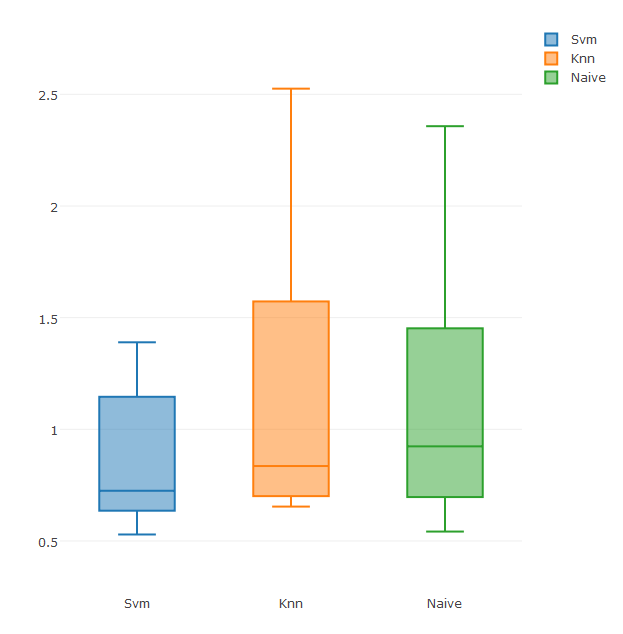
\includegraphics[width=\linewidth]{img/6mproxy1MASE.png}
\caption{Box plots of the MASE errors with the best parameters for the rolling window cross-validation with proxy 1.}
\end{figure}


\clearpage
\subsection{Proxy 2 results}
\begin{center}
\begin{tabular}{|c|c|c|c|}
\hline
& \multicolumn{3}{|c|}{\textbf{Proxy 2}} \\ \cline{2-4}
& \textbf{MSE} & \textbf{NMSE} & \textbf{MASE}          \\ \hline
Cost  & $2$            &$2^9$& $2^3$          \\ 
Gamma & $2^{-4}$ &$2^{-20}$& $2^{-6}$ \\ 
Error & $143.7454$ &$6.807685$& $2.742375$     \\ 
\hline
\end{tabular}


 \begin{figure}[!h]
\centering
\makebox[\linewidth]{%
\begin{subfigure}{.55\linewidth}
  \centering
  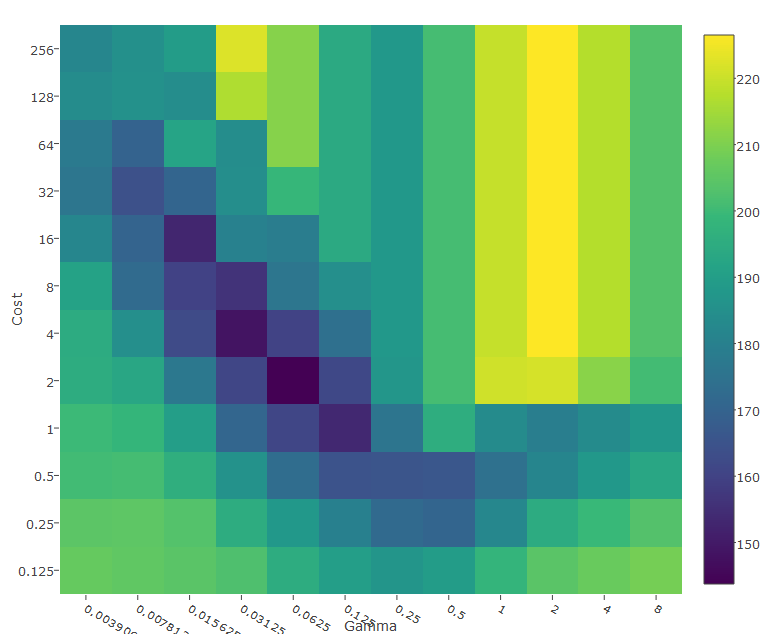
\includegraphics[width=\linewidth, height = 0.32\textheight]{img/6mMSEma.png}
  \caption{MSE using proxy 2.}
  \label{fig:heat11}
\end{subfigure}%
\begin{subfigure}{.55\linewidth}
  \centering
  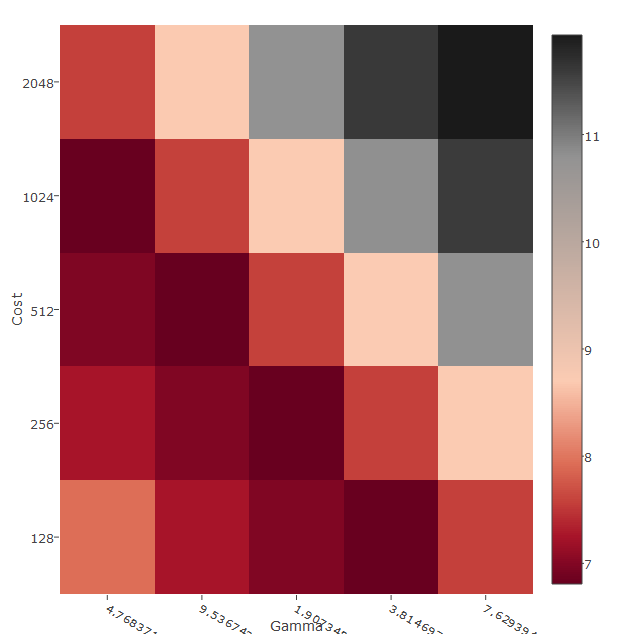
\includegraphics[width=\linewidth, height = 0.32\textheight]{img/6mNMSEma.png}
  \caption{NMSE using proxy 2.}
  \label{fig:heat22}
\end{subfigure}}
  \centering
  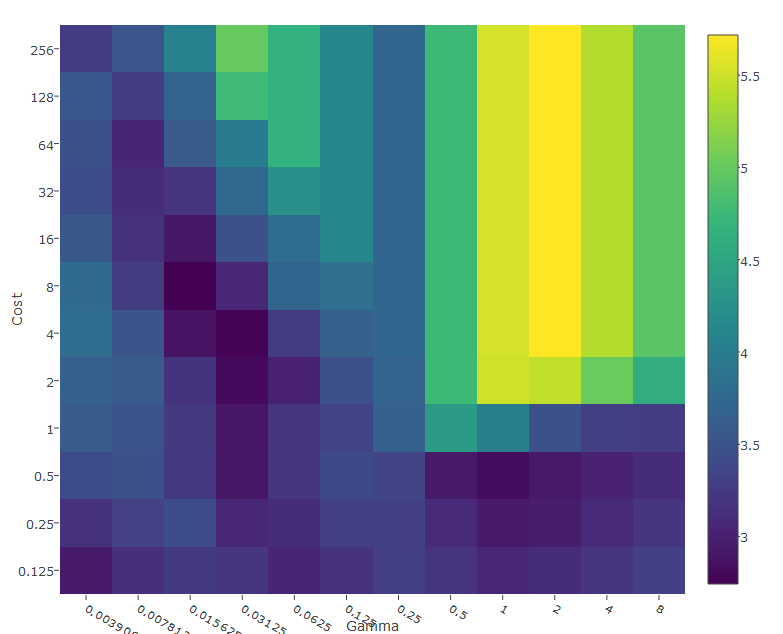
\includegraphics[width=0.6\linewidth, height = 0.34\textheight]{img/6mMASEma.png}
  \caption{MASE using proxy 2.}
  \label{fig:heat33}
\caption{Heat maps resulting of the SVM grid search for each error using proxy 2.}
\label{fig:heat6mp2}
\end{figure}\end{center}


\clearpage
\begin{figure}[!h]
\centering
\begin{tabular}{|c|c|c|}
   \hline
   & \multicolumn{2}{|c|}{\textbf{MSE}} \\ \cline{2-3}
   & \textbf{Errors} & \textbf{Parameters}          \\ \hline
   SVM  & $143.7454$        & $C = 2$, $\gamma = 2^{-4}$          \\ 
   KNN & $168.642$ & $K = 1$ \\ 
   Naive & $306.892442$ &      \\ 
   \hline
   \end{tabular}
\caption{Comparison of MSE errors with the best parameters configurations.}
\label{fig:table6mMSEp2}
\centering
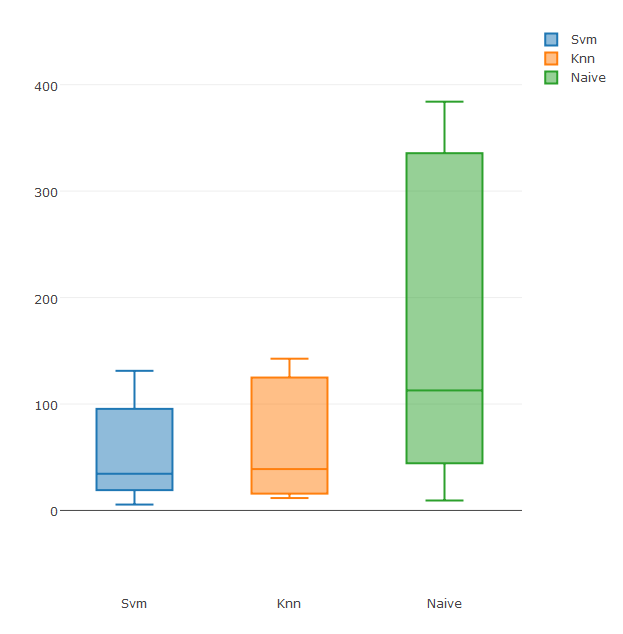
\includegraphics[width=\linewidth]{img/6mproxy2MSE.png}
\caption{Box plots of the MSE errors with the best parameters for the rolling window cross-validation with proxy 2.}
\end{figure}


\begin{figure}[!h]
\centering
\begin{tabular}{|c|c|c|}
   \hline
   & \multicolumn{2}{|c|}{\textbf{NMSE}} \\ \cline{2-3}
   & \textbf{Errors} & \textbf{Parameters}          \\ \hline
   SVM  & $6.807685$        & $C = 2^9$, $\gamma = 2^{-20}$          \\ 
   KNN & $7.031129$ & $K = 4$ \\ 
   Naive & $34.60042$ &      \\ 
   \hline
   \end{tabular}
\caption{Comparison of NMSE errors with the best parameters configurations.}
\label{fig:table6mNMSEp2}
\centering
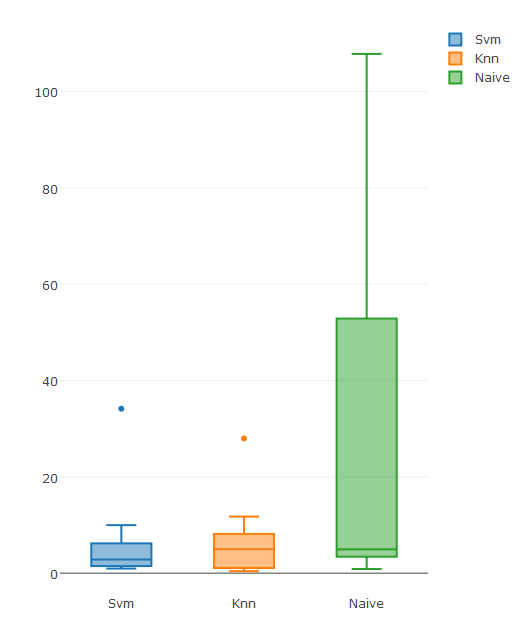
\includegraphics[width=\linewidth]{img/6mproxy2NMSE.png}
\caption{Box plots of the NMSE errors with the best parameters for the rolling window cross-validation with proxy 2.}
\end{figure}


\begin{figure}[!h]
\centering
\begin{tabular}{|c|c|c|}
   \hline
   & \multicolumn{2}{|c|}{\textbf{MASE}} \\ \cline{2-3}
   & \textbf{Errors} & \textbf{Parameters}          \\ \hline
   SVM  & $2.742375$        & $C = 2^3$, $\gamma = 2^{-6}$          \\ 
   KNN & $3.0839$ & $K = 4$ \\ 
   Naive & $6.477913$ &      \\ 
   \hline
   \end{tabular}
\caption{Comparison of MASE errors with the best parameters configurations.}
\label{fig:table6mMASEp2}
\centering
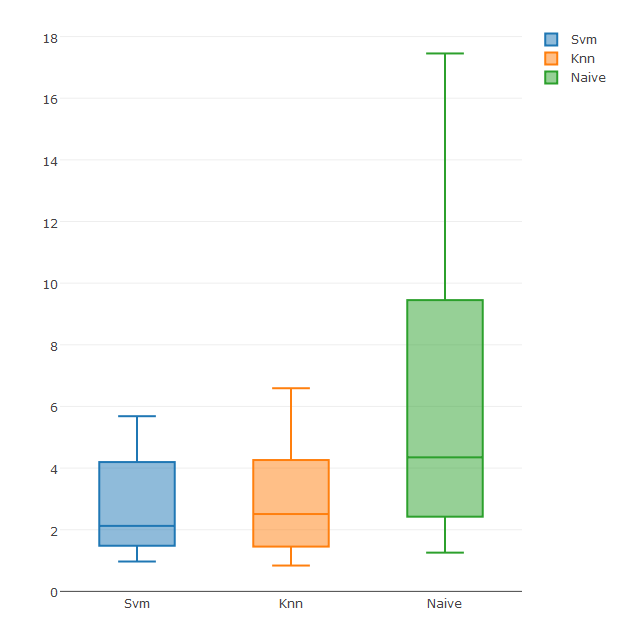
\includegraphics[width=\linewidth]{img/6mproxy2MASE.png}
\caption{Box plots of the MASE errors with the best parameters for the rolling window cross-validation with proxy 2.}
\end{figure}



\clearpage
\section{Longer history}

Then, I ran the experiment on a 10 years history. One will find on figure \ref{fig:plot10y} the plots of the time series with the applied proxies.


\begin{figure}[!h]
\centering
\makebox[\linewidth]{%
\begin{subfigure}{.6\linewidth}
  \centering
  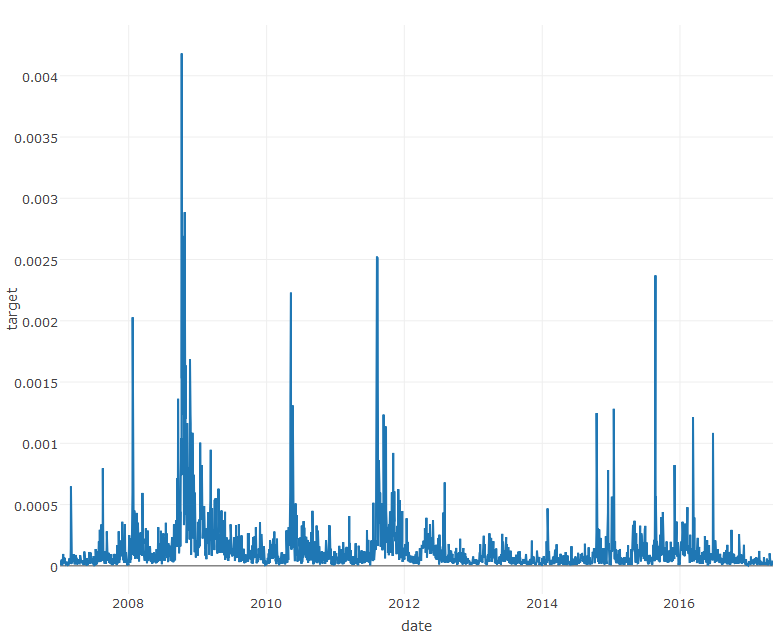
\includegraphics[width=\linewidth]{img/plot10sigma.png}
  \caption{Using proxy 1.}
  \label{fig:sub2.1}
\end{subfigure}%
\begin{subfigure}{.6\linewidth}
  \centering
  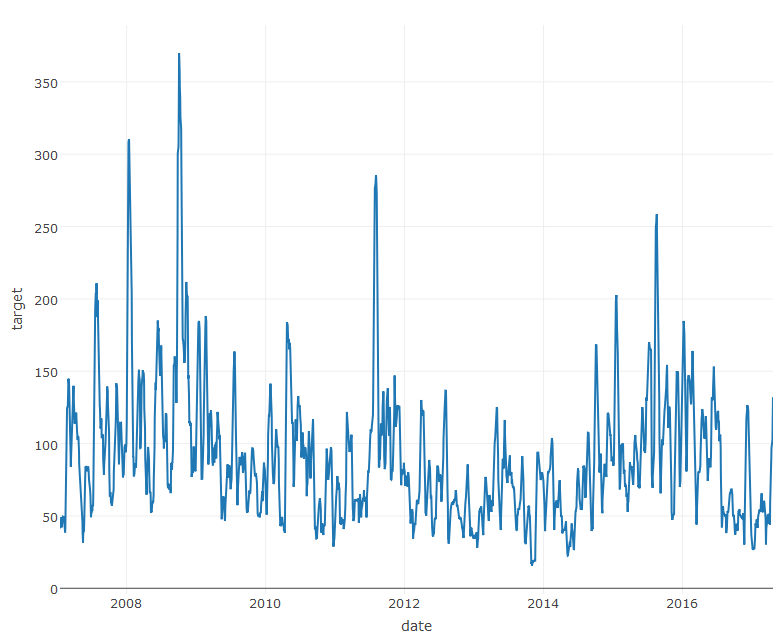
\includegraphics[width=\linewidth]{img/plot10ma.png}
  \caption{Using proxy 2.}
  \label{fig:sub2.2}
\end{subfigure}}
\caption{Plots of the longer time series using the two proxies.}
\label{fig:plot10y}
\end{figure}


One will find in the rest of this section, first the results using proxy 1, then the results using proxy 2.

The results of the search grid for the SVM parameters can be visualised on the heat maps on figure \ref{fig:heat10yp1} for proxy 1, and \ref{fig:heat10yp2} for proxy 2, where the resulting errors are displayed according to the parameters. The complete numeric results of the search grids can be found in appendix \ref{10yapp}. 

In the same way as for the reduced history heat maps, one can see on the heat maps that the most optimal cost and gamma parameters seem to lie on a diagonal.

Then, for each proxy, one will find the results of the experiments for SVM, KNN and the naive method regrouped for each error measure.

The results follow the same structure as those of the reduced history.



\clearpage
\begin{center}
\begin{tabular}{|c|c|c|c|}
\hline
& \multicolumn{3}{|c|}{\textbf{Proxy 1}} \\ \cline{2-4}
& \textbf{MSE} & \textbf{NMSE} & \textbf{MASE} \\ \hline
Cost  &  $2^{-3}$        & $2^{18}$    & $2^{12}$       \\ 
Gamma &  $2^{-10}$       & $2^{-11}$   & $2^{-10}$      \\ 
Error &  $2.965806e-09$  & $3.969722$  & $1.716571$     \\ 
\hline
\end{tabular}


 \begin{figure}[!h]
\centering
\makebox[\linewidth]{%
\begin{subfigure}{.6\linewidth}
  \centering
  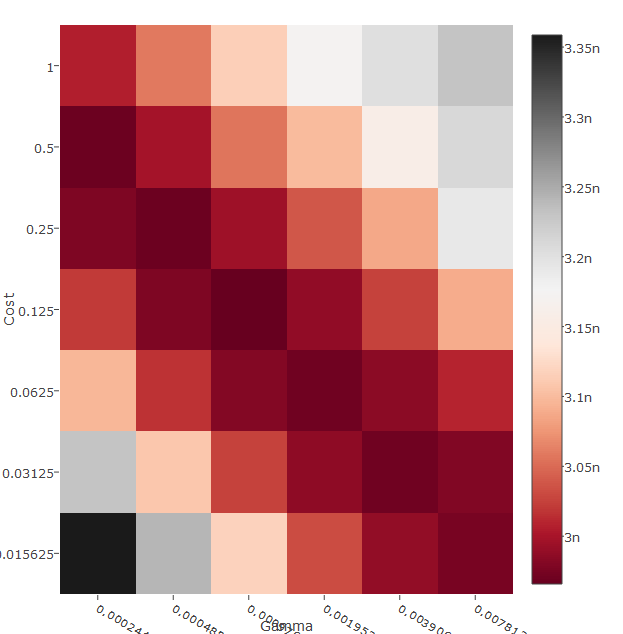
\includegraphics[width=\linewidth, height = 0.33\textheight]{img/10yMSEsigma.png}
  \caption{MSE using proxy 1.}
  \label{fig:heat1a}
\end{subfigure}%
\begin{subfigure}{.6\linewidth}
  \centering
  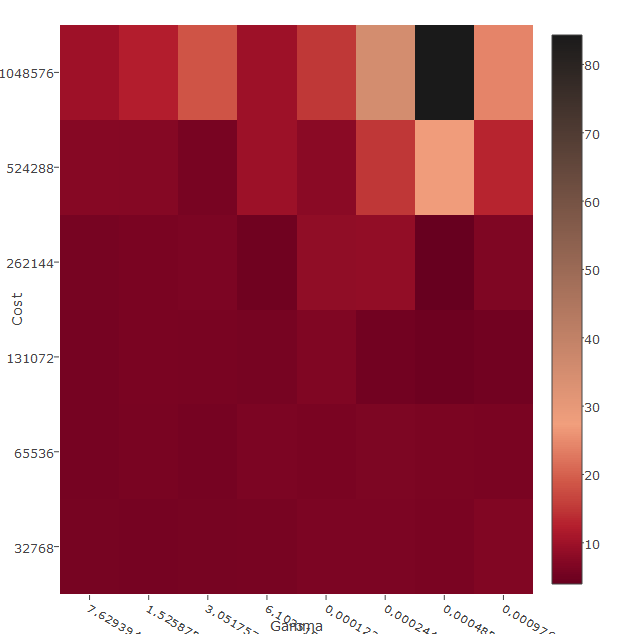
\includegraphics[width=\linewidth, height = 0.33\textheight]{img/10yNMSEsigma.png}
  \caption{NMSE using proxy 1.}
  \label{fig:heat2a}
\end{subfigure}}
  \centering
  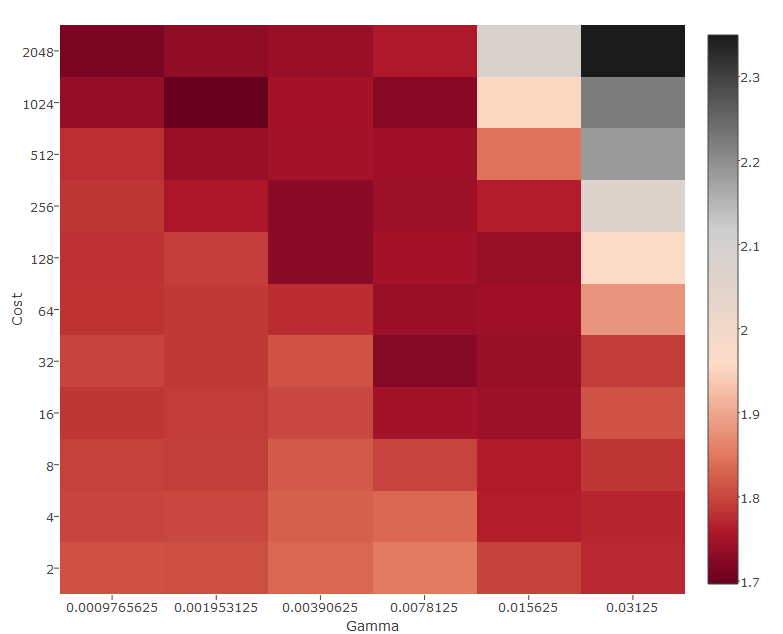
\includegraphics[width=0.65\linewidth, height = 0.35\textheight]{img/10yMASEsigma.png}
  \caption{MASE using proxy 1.}
  \label{fig:heat3a}
\caption{Heat maps resulting of the SVM grid search for each error using proxy 1.}
\label{fig:heat10yp1}
\end{figure}\end{center}


\clearpage
\subsection{Proxy 1 results}
\begin{figure}[!h]
\centering
\begin{tabular}{|c|c|c|}
   \hline
   & \multicolumn{2}{|c|}{\textbf{MSE}} \\ \cline{2-3}
   & \textbf{Errors} & \textbf{Parameters}          \\ \hline
   SVM  & $2.965806e-09$  & $C = 2^{-3}$, $\gamma = 2^{-10}$ \\ 
   KNN & $2.87505e-09$ & $K = 14 $ \\ 
   Naive & $4.738385e-09$  &      \\ 
   \hline
   \end{tabular}
\caption{Comparison of MSE errors with the best parameters configurations.}
\label{fig:table10yMSEp1}
\centering
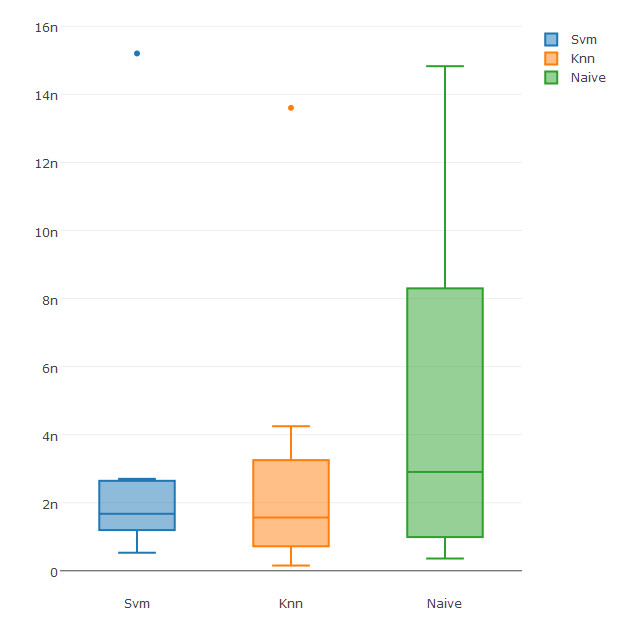
\includegraphics[width=\linewidth]{img/10yproxy1MSE.png}
\caption{Box plots of the MSE errors with the best parameters for the rolling window cross-validation with proxy 1. On the ordinates, $n$ represents $n := 10^{-9}$.}\label{fig:table10yMSEp1a}
\end{figure}


\begin{figure}[!h]
\centering
\begin{tabular}{|c|c|c|}
   \hline
   & \multicolumn{2}{|c|}{\textbf{NMSE}} \\ \cline{2-3}
   & \textbf{Errors} & \textbf{Parameters}          \\ \hline
   SVM  &  $3.969722$      & $C = 2^{18}$, $\gamma = 2^{-11}$          \\ 
   KNN & $5.32743$  & $K = 12$ \\ 
   Naive & $15.23972$ &      \\ 
   \hline
   \end{tabular}
\caption{Comparison of NMSE errors with the best parameters configurations.}
\label{fig:table10yNMSEp1}
\centering
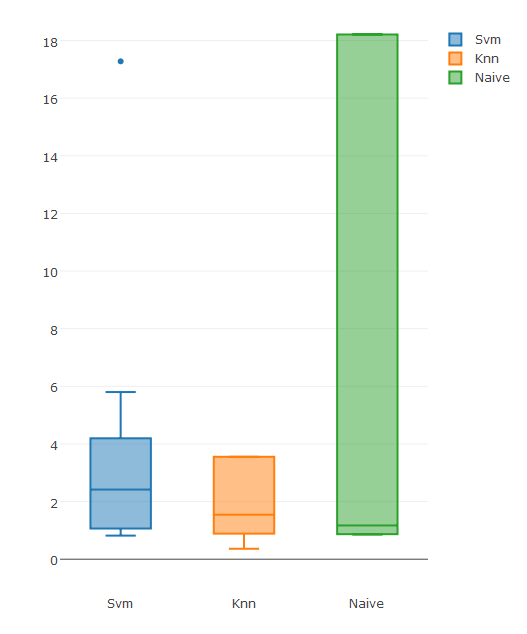
\includegraphics[width=\linewidth]{img/10yproxy1NMSE.png}
\caption{Box plots of the NMSE errors with the best parameters for the rolling window cross-validation with proxy 1.}\label{fig:table10yNMSEp1a}
\end{figure}


\begin{figure}[!h]
\centering
\begin{tabular}{|c|c|c|}
   \hline
   & \multicolumn{2}{|c|}{\textbf{MASE}} \\ \cline{2-3}
   & \textbf{Errors} & \textbf{Parameters}          \\ \hline
   SVM  &  $1.716571$       & $C = 2^{12}$, $\gamma = 2^{-10}$ \\ 
   KNN & $1.619784$ & $K = 12$ \\ 
   Naive & $2.808507$ &      \\ 
   \hline
   \end{tabular}
\caption{Comparison of MASE errors with the best parameters configurations.}
\label{fig:table10yMASEp1}
\centering
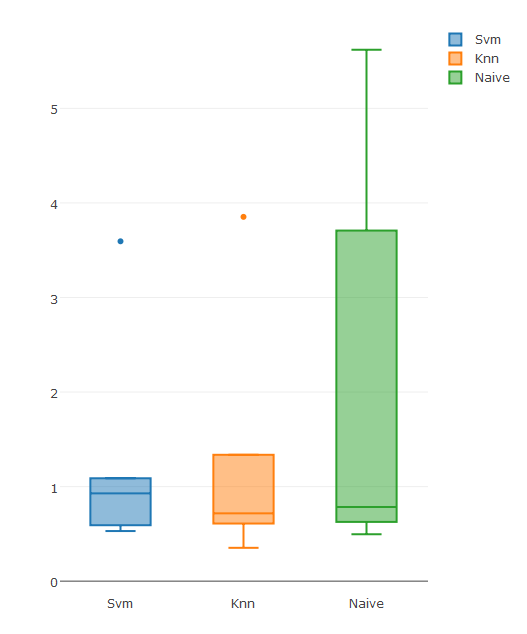
\includegraphics[width=\linewidth]{img/10yproxy1MASE.png}
\caption{Box plots of the MASE errors with the best parameters for the rolling window cross-validation with proxy 1.}
\end{figure}


\clearpage
\begin{center}
\begin{tabular}{|c|c|c|c|}
\hline
& \multicolumn{3}{|c|}{\textbf{Proxy 2}} \\ \cline{2-4}
& \textbf{MSE} & \textbf{NMSE} & \textbf{MASE}          \\ \hline
Cost  & $2^{10}$    &$2^{13}$ & $2^{11}$     \\ 
Gamma & $2^{-15}$   &$2^{-16}$& $2^{-13}$     \\ 
Error & $472.1264$ &$65.12693$& $6.706905$     \\ 
\hline
\end{tabular}
 \begin{figure}[!h]
\centering
\makebox[\linewidth]{%
\begin{subfigure}{.55\linewidth}
  \centering
  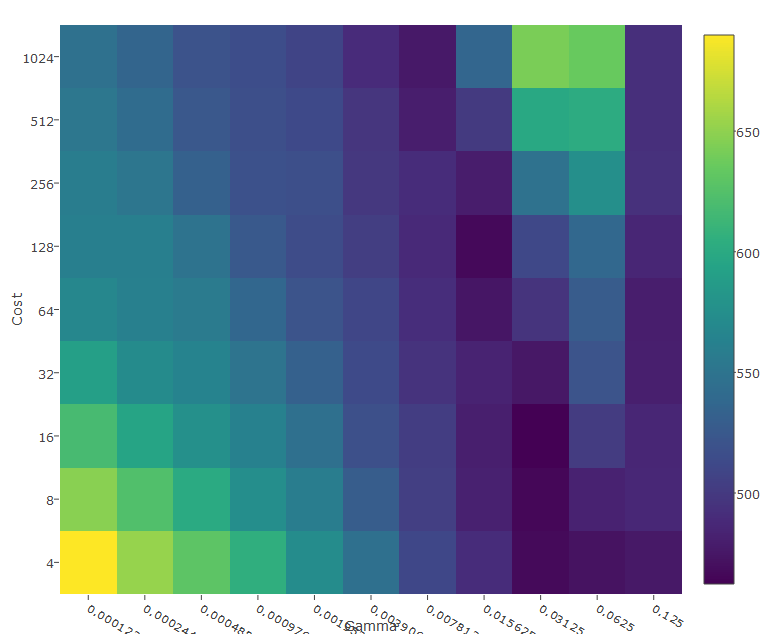
\includegraphics[width=\linewidth, height = 0.33\textheight]{img/10yMSEma.png}
  \caption{MSE using proxy 2.}
  \label{fig:heat11a}
\end{subfigure}%
\begin{subfigure}{.55\linewidth}
  \centering
  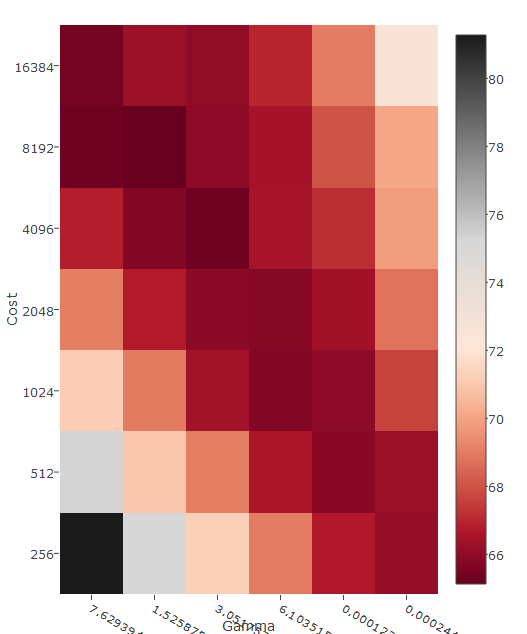
\includegraphics[width=\linewidth, height = 0.33\textheight]{img/10yNMSEma.png}
  \caption{NMSE using proxy 2.}
  \label{fig:heat22a}
\end{subfigure}}
  \centering
  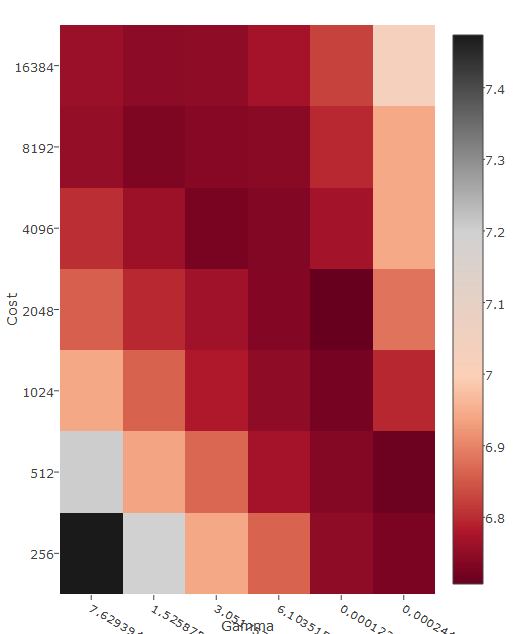
\includegraphics[width=0.55\linewidth, height = 0.33\textheight]{img/10yMASEma.png}
  \caption{MASE using proxy 2.}
  \label{fig:heat33a}
\caption{Heat maps resulting of the SVM grid search for each error using proxy 2.}
\label{fig:heat10yp2}
\end{figure}\end{center}


\clearpage
\subsection{Proxy 2 results}
\begin{figure}[!h]
\centering
\begin{tabular}{|c|c|c|}
   \hline
   & \multicolumn{2}{|c|}{\textbf{MSE}} \\ \cline{2-3}
   & \textbf{Errors} & \textbf{Parameters}          \\ \hline
   SVM  &  $472.1264$  & $C = 2^{10}$, $\gamma = 2^{-15}$          \\ 
   KNN & $720.085$  & $K = 6$ \\ 
   Naive & $2223.865$  &      \\ 
   \hline
   \end{tabular}
\caption{Comparison of MSE errors with the best parameters configurations.}
\label{fig:table10yMSEp2}
\centering
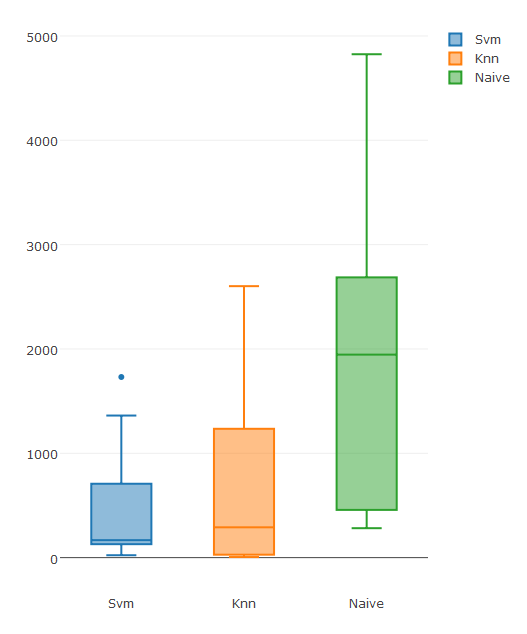
\includegraphics[width=0.95\linewidth, height = 0.67\textheight]{img/10yproxy2MSE.png}
\caption{Box plots of the MSE errors with the best parameters for the rolling window cross-validation with proxy 2.}
\end{figure}


\begin{figure}[!h]
\centering
\begin{tabular}{|c|c|c|}
   \hline
   & \multicolumn{2}{|c|}{\textbf{NMSE}} \\ \cline{2-3}
   & \textbf{Errors} & \textbf{Parameters}          \\ \hline
   SVM  &  $65.12693$  & $C = 2^{13}$, $\gamma = 2^{-16}$          \\ 
   KNN & $120.5991$  & $K = 3$ \\ 
   Naive & $281.0051$ &      \\ 
   \hline
   \end{tabular}
\caption{Comparison of NMSE errors with the best parameters configurations.}
\label{fig:table10yNMSEp2}
\centering
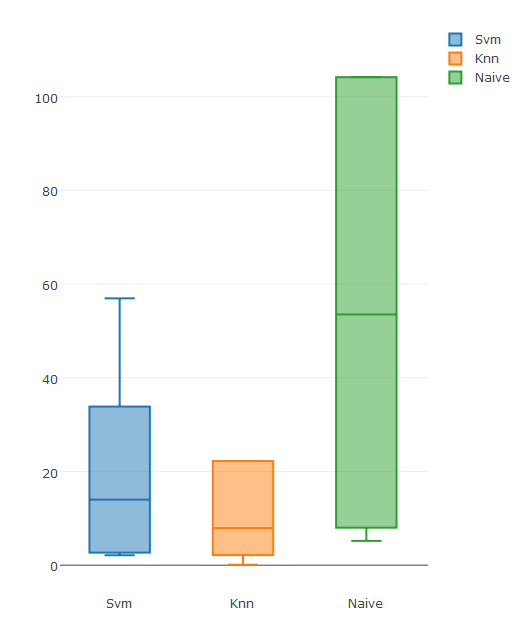
\includegraphics[width=\linewidth]{img/10yproxy2NMSE.png}
\caption{Box plots of the NMSE errors with the best parameters for the rolling window cross-validation with proxy 2.}
\end{figure}


\begin{figure}[!h]
\centering
\begin{tabular}{|c|c|c|}
   \hline
   & \multicolumn{2}{|c|}{\textbf{MASE}} \\ \cline{2-3}
   & \textbf{Errors} & \textbf{Parameters}          \\ \hline
   SVM  & $6.706905$& $C = 2^{11}$, $\gamma = 2^{-13}$          \\ 
   KNN & $10.30528$ & $K = 6$ \\ 
   Naive & $18.31019$ &      \\ 
   \hline
   \end{tabular}
\caption{Comparison of MASE errors with the best parameters configurations.}
\label{fig:table10yMASEp2}
\centering
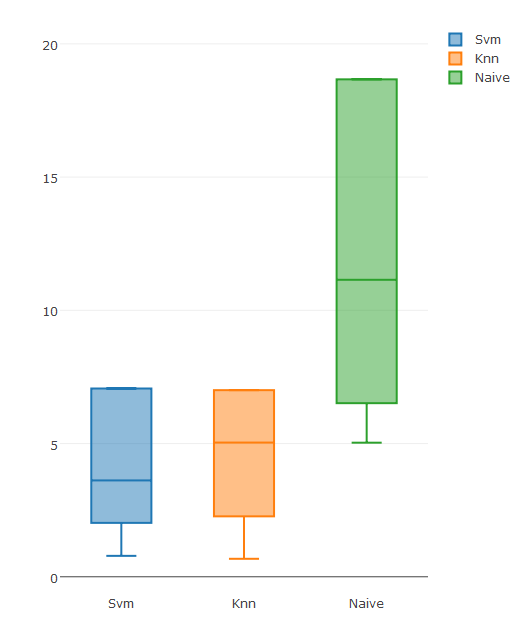
\includegraphics[width=\linewidth]{img/10yproxy2MASE.png}
\caption{Box plots of the MASE errors with the best parameters for the rolling window cross-validation with proxy 2.}
\end{figure}



\clearpage
\section{Discussion}


First we will have a look at the optimal parameters for each algorithm, proxy and history length. We will try to see if there is any tendency or if any parameters are constant regardless of the proxy,... Then we will compare the actual errors measures for each algorithm to see if there's one that is constantly performing better than the others.

\subsection{Optimal parameters}
On figures \ref{fig:comparep1} and \ref{fig:comparep2} one can find the optimal parameters for each case. 

For KNN, we observe that the best choice for the $k$ parameter for proxy 1 is between 12 and 15, while for proxy 2 it is between 1 and 6. 
This is an expected result due to the nature of both series. Indeed, the smoothness of proxy 2 makes the very nearest neighbors the best choice, while for proxy 1, a larger pool of neighbors might be more suitable.

Regarding SVM, we already had observed that the best parameters laid on a diagonal. Therefore, while this results were found optimal, choosing $C$ slightly bigger and $\gamma$ slightly smaller could also do the trick. By observation, we can see that $C$ ranges from $2^{-3}$ to $2^{18}$ and $\gamma$ ranges from $2^{-20}$ to $2^{-4}$. Tough, we can not conclude of any combination of parameters being optimal in all cases. 

\begin{figure}[!h]
\centering
\begin{tabular}{|c|c|c|c|}
\hline
    & \multicolumn{3}{|c|}{\textbf{Reduced history}} \\ \cline{2-4}
    & \textbf{MSE} & \textbf{NMSE} & \textbf{MASE}          \\ \hline
    SVM  & $C = 2$, $\gamma = 2^{-13}$&  $C = 2^9$, $\gamma = 2^{-19}$& $C = 2^8$, $\gamma = 2^{-17}$ \\ 
    KNN & $15$ &$15$ &$15$         \\ 
    \hline
\multicolumn{4}{c}{\textbf{}} \\ \cline{1-4}
    & \multicolumn{3}{|c|}{\textbf{Longer history}} \\ \cline{2-4}
    & \textbf{MSE} & \textbf{NMSE} & \textbf{MASE}          \\ \hline
    SVM  & $C = 2^{-3}$, $\gamma = 2^{-10}$  & $C = 2^{18}$, $\gamma = 2^{-11}$&  $C = 2^{12}$, $\gamma = 2^{-10}$ \\ 
    KNN & $14$ &$12$ &$12$         \\ \hline
\end{tabular}
\caption{Comparison of the results between the models' parameters using proxy 1.}
\label{fig:comparep1}
\end{figure}

\begin{figure}[!h]
\centering
\begin{tabular}{|c|c|c|c|}
\hline
    & \multicolumn{3}{|c|}{\textbf{Reduced history}} \\ \cline{2-4}
    & \textbf{MSE} & \textbf{NMSE} & \textbf{MASE}          \\ \hline
    SVM  & $C = 2$, $\gamma = 2^{-4}$&  $C = 2^9$, $\gamma = 2^{-20}$& $C = 2^3$, $\gamma = 2^{-6}$ \\ 
    KNN & $1$ &$4$ &$4$         \\ 
    \hline
\multicolumn{4}{c}{\textbf{}} \\ \cline{1-4}
    & \multicolumn{3}{|c|}{\textbf{Longer history}} \\ \cline{2-4}
    & \textbf{MSE} & \textbf{NMSE} & \textbf{MASE}          \\ \hline
    SVM  & $C = 2^{10}$, $\gamma = 2^{-15}$  & $C = 2^{13}$, $\gamma = 2^{-16}$&  $C = 2^{11}$, $\gamma = 2^{-13}$ \\ 
    KNN & $6$ &$3$ &$6$         \\ \hline
\end{tabular}
\caption{Comparison of the results between the models' parameters using proxy 2.}
\label{fig:comparep2}
\end{figure}


\subsection{Error measures}

Now that we have all the results for the optimal parameters of the models, it is time to compare the models between them.

The first observation that I should point out is that, looking on figures \ref{fig:compare6m} and \ref{fig:compare10y}, regarding the MASE error measure, the proxy 1 is systematically providing much better results. Regarding MSE and NMSE, we can't make any deductions between the proxies. 

\begin{figure}[!h]
\centering
\begin{minipage}{\textwidth}
\begin{minipage}{0.5\textwidth}
\begin{center}
\vskip10pt
   \begin{footnotesize}
   \begin{tabular}{|c|c|c|c|}
   \hline
   & \multicolumn{3}{|c|}{\textbf{Proxy 1}} \\ \cline{2-4}
   & \textbf{MSE}  & \textbf{NMSE} & \textbf{MASE}          \\ \hline
   SVM  & $5.443549e-10$ &$5.098590$& $1.2278$         \\ 
   KNN & $6.492108e-10$ &$7.424236$& $1.518099$ \\ 
   Naive & $6.144618e-10$ &$7.059421$& $1.483807$     \\ 
   \hline
   \end{tabular}
   \end{footnotesize}
\end{center}
\end{minipage}
\begin{minipage}{0.5\textwidth}
\begin{center}
\vskip12pt
   \begin{footnotesize}
   \begin{tabular}{|c|c|c|c|}
   \hline
   & \multicolumn{3}{|c|}{\textbf{Proxy 2}} \\ \cline{2-4}
   & \textbf{MSE}  & \textbf{NMSE} & \textbf{MASE}          \\ \hline
   SVM  & $143.7454$      &$6.807685$& $2.742375$         \\ 
   KNN & $168.642$     &$7.031129$& $3.0839$ \\ 
   NAIVE & $306.892442$ &$34.60042$& $6.477913$      \\ 
   \hline
   \end{tabular}
   \end{footnotesize}
\end{center}
\end{minipage}
\end{minipage}
\caption{Comparison of the results between the models for the reduced history.}
\label{fig:compare6m}
\end{figure}

\begin{figure}[!h]
\centering
\begin{minipage}{\textwidth}
\begin{minipage}{0.5\textwidth}
\begin{center}
\vskip10pt
   \begin{footnotesize}
   \begin{tabular}{|c|c|c|}
   \hline
   & \multicolumn{2}{|c|}{\textbf{Proxy 1}} \\ \cline{2-3}
   & \textbf{MSE} & \textbf{MASE}          \\ \hline
   SVM  & $1.969437e-09$ & $1.696371$         \\ 
   KNN & $2.929323e-09$ & $1.679673$ \\ 
   Naive & $4.443686e-09$ & $2.821883$     \\ 
   \hline
   \end{tabular}
   \end{footnotesize}
\end{center}
\end{minipage}
\begin{minipage}{0.5\textwidth}
\begin{center}
\vskip12pt
   \begin{footnotesize}
   \begin{tabular}{|c|c|c|}
   \hline
   & \multicolumn{2}{|c|}{\textbf{Proxy 2}} \\ \cline{2-3}
   & \textbf{MSE} & \textbf{MASE}          \\ \hline
   SVM  & $462.2867$      & $7.885050$         \\ 
   KNN & $388.4074$      & $8.400853$ \\ 
   NAIVE & $1213.68939$      & $25.98904$      \\ 
   \hline
   \end{tabular}
   \end{footnotesize}
\end{center}
\end{minipage}
\end{minipage}
\caption{Comparison of the results between the models for the longer history.}
\label{fig:compare10y}
\end{figure}

Regarding MSE and MASE, SVM shows the best results when using proxy 2, but it is unclear regarding proxy 1. Indeed, the results for the longer history shows slightly better results for KNN. If we take a closer look at the box-plots on figure \ref{fig:table10yMSEp1a} we can see that the median is slightly lower for KNN, but the box is smaller for SVM. Even for NMSE of proxy 1 of the longer history, as one can see on figure \ref{fig:table10yNMSEp1a}, the box for KNN seems lower on all quartiles. We might be inclined to conclude that when using proxy 1, KNN is the better choice. Although on the reduced history KNN does not show the best results, the longer history is a better generalisation of the problem.

Regarding NMSE, SVM shows strictly better results in all cases compared to the other algorithms.










\chapter{Conclusion \& Future Work }


\section{Conclusion}


\section{Future work}

New experiments can be conducted in order to strengthen our results. One can search the optimal parameters on a larger pool of financial time series and compare the results with the established ones.

Regarding the tool, new algorithms could be added. The interface could be improved in order to let the user choose a personal file as a data set input.

A research on trading strategies could be interesting. Add new practical functionalities to the tool such as agents simulating trading strategies could be the next step.



\clearpage
\appendix
\chapter{Search grid on reduced history}\label{6mapp}

\begin{table}[h!]
\centering
\begin{adjustbox}{width=\textwidth}
\begin{tabular}{|r|r|rrrrrr|}
\hline
\multicolumn{8}{|c|}{GAMMA} \tabularnewline
\hline
  &MSE&  2\verb|^|-14 & 2\verb|^|-13 & 2\verb|^|-12 & 2\verb|^|-11 & 2\verb|^|-10 & 2\verb|^|-9 \\ 
  \hline
  &2\verb|^|-4 & 5.514144E-10 & 5.514746E-10 & 5.513528E-10 & 5.504903E-10 & 5.480246E-10 & 5.453717E-10 \\ 
  C&2\verb|^|-3 & 5.514747E-10 & 5.513525E-10 & 5.504747E-10 & 5.479189E-10 & 5.452817E-10 & 5.447209E-10 \\ 
  O&2\verb|^|-2 & 5.513524E-10 & 5.504670E-10 & 5.478657E-10 & 5.451697E-10 & 5.444985E-10 & 5.451554E-10 \\ 
  S&2\verb|^|-1 & 5.504632E-10 & 5.478390E-10 & 5.450924E-10 & 5.444111E-10 & 5.451489E-10 & 5.541286E-10 \\ 
  T&2\verb|^|0 & 5.478257E-10 & 5.450938E-10 & 5.443789E-10 & 5.452819E-10 & 5.540381E-10 & 5.590476E-10 \\ 
  &2\verb|^|1 & 5.450847E-10 & 5.443549E-10 & 5.452804E-10 & 5.539904E-10 & 5.577905E-10 & 5.858172E-10 \\ 
  &2\verb|^|2 & 5.443690E-10 & 5.453142E-10 & 5.540757E-10 & 5.574863E-10 & 5.870562E-10 & 6.275414E-10 \\ 
   \hline
\end{tabular}
\end{adjustbox}
\caption{Shortened results of the search grid for the SVM parameters for a period of 6 months with MSE using proxy 1.}
\end{table}

\begin{table}[h!]
\centering
\begin{adjustbox}{width=\textwidth}
\begin{tabular}{|r|r|rrrrr|}
\hline
\multicolumn{7}{|c|}{GAMMA} \tabularnewline
 \hline
 &NMSE& 2\verb|^|-21 & 2\verb|^|-20 & 2\verb|^|-19 & 2\verb|^|-18 & 2\verb|^|-17 \\ 
  \hline
  &2\verb|^|7 & 6.84836 & 6.57169 & 6.19614 & 5.81115 & 5.09916 \\ 
  C&2\verb|^|8 & 6.57278 & 6.19589 & 5.80985 & 5.09860 & 5.14298 \\ 
  O&2\verb|^|9 & 6.19391 & 5.81197 & \textbf{5.09859} & 5.14255 & 5.85501 \\ 
  S&2\verb|^|10 & 5.81219 & 5.10674 & 5.14560 & 5.84833 & 7.45604 \\ 
  T&2\verb|^|11 & 5.11337 & 5.14240 & 5.84387 & 7.45500 & 8.22528 \\ 
   \hline
\end{tabular}
\end{adjustbox}
\caption{Shortened results of the search grid for the SVM parameters for a period of 9 months with NMSE using proxy 1.}
\end{table}

\begin{table}[h!]
\centering
\begin{adjustbox}{width=\textwidth}
\begin{tabular}{|r|r|rrrrrr|}
\hline
\multicolumn{8}{|c|}{GAMMA} \tabularnewline
\hline
 &MASE& 2\verb|^|-19 & 2\verb|^|-18 & 2\verb|^|-17 & 2\verb|^|-16 & 2\verb|^|-15 & 2\verb|^|-14 \\ 
  \hline
  &2\verb|^|5 & 1.394230E+00 & 1.372780E+00 & 1.341575E+00 & 1.299343E+00 & 1.237166E+00 & 1.228156E+00 \\ 
  C&2\verb|^|6 & 1.372800E+00 & 1.341597E+00 & 1.299363E+00 & 1.237127E+00 & 1.228308E+00 & 1.278435E+00 \\ 
  O&2\verb|^|7 & 1.341543E+00 & 1.299340E+00 & 1.236950E+00 & 1.228114E+00 & 1.277950E+00 & 1.367800E+00 \\ 
  S&2\verb|^|8 & 1.299224E+00 & \textbf{1.236896E+00} & 1.227800E+00 & 1.277370E+00 & 1.368960E+00 & 1.407855E+00 \\ 
  T&2\verb|^|9 & 1.236821E+00 & 1.227806E+00 & 1.278154E+00 & 1.368133E+00 & 1.407725E+00 & 1.424985E+00 \\ 
  &2\verb|^|10 & 1.228114E+00 & 1.277693E+00 & 1.369221E+00 & 1.407579E+00 & 1.422009E+00 & 1.421993E+00 \\ 
   \hline
\end{tabular}
\end{adjustbox}
\caption{Results of the search grid for the SVM parameters for a period of 6 months with MASE using proxy 1.}
\end{table}

\begin{table}[h!]
\centering
\begin{adjustbox}{width=\textwidth}
\begin{tabular}{|r|r|rrrrrrrrrrrr|}
\hline
\multicolumn{14}{|c|}{GAMMA} \tabularnewline
 \hline
 &MSE& 2\verb|^|-8 & 2\verb|^|-7 & 2\verb|^|-6 & 2\verb|^|-5 & 2\verb|^|-4 & 2\verb|^|-3 & 2\verb|^|-2 & 2\verb|^|-1 & 2\verb|^|0 & 2\verb|^|1 & 2\verb|^|2 & 2\verb|^|3 \\ 
  \hline
  &2\verb|^|-3 & 206.42 & 205.45 & 204.38 & 202.38 & 195.14 & 189.98 & 186.85 & 189.34 & 197.84 & 204.31 & 206.99 & 208.91 \\ 
  &2\verb|^|-2 & 204.64 & 205.01 & 203.25 & 195.02 & 187.86 & 179.88 & 172.13 & 170.49 & 182.20 & 194.62 & 199.35 & 203.15 \\ 
  &2\verb|^|-1 & 200.63 & 200.97 & 195.95 & 185.77 & 173.25 & 164.91 & 165.62 & 166.12 & 174.49 & 181.69 & 187.72 & 192.85 \\ 
  C&2\verb|^|0 & 199.80 & 198.27 & 190.01 & 170.71 & 160.93 & 153.49 & 176.02 & 195.43 & 183.80 & 179.22 & 183.50 & 187.55 \\ 
  O&2\verb|^|1 & 194.98 & 192.87 & 176.83 & 161.06 & \textbf{143.75} & 161.55 & 186.98 & 201.08 & 220.66 & 221.42 & 211.50 & 200.74 \\ 
  S&2\verb|^|2 & 194.78 & 185.00 & 162.29 & 148.48 & 160.04 & 173.97 & 187.93 & 201.10 & 219.42 & 226.53 & 217.30 & 202.99 \\ 
  T&2\verb|^|3 & 191.29 & 172.47 & 159.88 & 156.11 & 176.38 & 184.86 & 187.93 & 201.10 & 219.42 & 226.53 & 217.30 & 202.99 \\ 
  &2\verb|^|4 & 181.92 & 170.10 & 152.84 & 180.04 & 178.63 & 193.97 & 187.93 & 201.10 & 219.42 & 226.53 & 217.30 & 202.99 \\ 
  &2\verb|^|5 & 176.33 & 164.16 & 170.39 & 184.49 & 198.91 & 193.97 & 187.93 & 201.10 & 219.42 & 226.53 & 217.30 & 202.99 \\ 
  &2\verb|^|6 & 177.71 & 169.77 & 191.88 & 184.24 & 211.09 & 193.97 & 187.93 & 201.10 & 219.42 & 226.53 & 217.30 & 202.99 \\ 
  &2\verb|^|7 & 184.15 & 185.53 & 184.38 & 216.65 & 211.09 & 193.97 & 187.93 & 201.10 & 219.42 & 226.53 & 217.30 & 202.99 \\ 
  &2\verb|^|8 & 181.79 & 185.21 & 189.34 & 222.38 & 211.09 & 193.97 & 187.93 & 201.10 & 219.42 & 226.53 & 217.30 & 202.99 \\ 
   \hline
\end{tabular}
\end{adjustbox}
\caption{Results of the search grid for the SVM parameters for a period of 6 months with MSE using proxy 2.}
\end{table}

\begin{table}[h!]
\centering
\begin{adjustbox}{width=\textwidth}
\begin{tabular}{|r|r|rrrrr|}
\hline
\multicolumn{7}{|c|}{GAMMA} \tabularnewline
   \hline
  &NMSE& 2\verb|^|-21 & 2\verb|^|-20 & 2\verb|^|-19 & 2\verb|^|-18 & 2\verb|^|-17 \\ 
  \hline
  &2\verb|^|7 & 7.9350 & 7.2498 & 6.9816 & 6.8122 & 7.5711 \\ 
  C&2\verb|^|8 & 7.2490 & 6.9824 & 6.8123 & 7.5698 & 8.7066 \\ 
  O&2\verb|^|9 & 6.9799 & \textbf{6.8077} & 7.5755 & 8.7088 & 10.8001 \\ 
  S&2\verb|^|10 & 6.8136 & 7.5730 & 8.7038 & 10.8136 & 11.5877 \\ 
  T&2\verb|^|11 & 7.5711 & 8.6949 & 10.7941 & 11.6053 & 11.9286 \\ 
   \hline
\end{tabular}
\end{adjustbox}
\caption{Shortened results of the search grid for the SVM parameters for a period of 9 months with NMSE using proxy 2.}
\end{table}

\begin{table}[h!]
\centering
\begin{adjustbox}{width=\textwidth}
\begin{tabular}{|r|r|rrrrrrrrrrrr|}
\hline
\multicolumn{14}{|c|}{GAMMA} \tabularnewline
\hline
    &MASE& 2\verb|^|-8 & 2\verb|^|-7 & 2\verb|^|-6 & 2\verb|^|-5 & 2\verb|^|-4 & 2\verb|^|-3 & 2\verb|^|-2 & 2\verb|^|-1 & 2\verb|^|0 & 2\verb|^|1 & 2\verb|^|2 & 2\verb|^|3 \\ 
  \hline
  &2\verb|^|-3 & 2.94 & 3.13 & 3.24 & 3.20 & 3.05 & 3.17 & 3.29 & 3.18 & 3.06 & 3.11 & 3.21 & 3.30 \\ 
  &2\verb|^|-2 & 3.16 & 3.32 & 3.43 & 3.06 & 3.11 & 3.29 & 3.31 & 3.09 & 2.94 & 2.96 & 3.09 & 3.20 \\ 
  &2\verb|^|-1 & 3.42 & 3.48 & 3.24 & 2.91 & 3.20 & 3.41 & 3.35 & 2.93 & 2.83 & 2.92 & 3.02 & 3.10 \\ 
  C&2\verb|^|0 & 3.59 & 3.50 & 3.23 & 2.90 & 3.20 & 3.34 & 3.64 & 4.38 & 4.02 & 3.48 & 3.29 & 3.28 \\ 
  O&2\verb|^|1 & 3.65 & 3.58 & 3.17 & 2.81 & 3.01 & 3.46 & 3.69 & 4.76 & 5.51 & 5.44 & 5.02 & 4.59 \\ 
  S&2\verb|^|2 & 3.81 & 3.51 & 2.88 & 2.75 & 3.26 & 3.66 & 3.73 & 4.76 & 5.53 & 5.72 & 5.38 & 4.92 \\ 
  T&2\verb|^|3 & 3.77 & 3.28 & \textbf{2.74} & 3.06 & 3.71 & 3.85 & 3.73 & 4.76 & 5.53 & 5.72 & 5.38 & 4.92 \\ 
  &2\verb|^|4 & 3.56 & 3.16 & 2.91 & 3.47 & 3.81 & 4.13 & 3.73 & 4.76 & 5.53 & 5.72 & 5.38 & 4.92 \\ 
  &2\verb|^|5 & 3.43 & 3.11 & 3.19 & 3.76 & 4.25 & 4.13 & 3.73 & 4.76 & 5.53 & 5.72 & 5.38 & 4.92 \\ 
  &2\verb|^|6 & 3.48 & 3.05 & 3.59 & 3.99 & 4.66 & 4.13 & 3.73 & 4.76 & 5.53 & 5.72 & 5.38 & 4.92 \\ 
  &2\verb|^|7 & 3.55 & 3.28 & 3.68 & 4.76 & 4.66 & 4.13 & 3.73 & 4.76 & 5.53 & 5.72 & 5.38 & 4.92 \\ 
  &2\verb|^|8 & 3.26 & 3.53 & 4.05 & 5.00 & 4.66 & 4.13 & 3.73 & 4.76 & 5.53 & 5.72 & 5.38 & 4.92 \\ 
   \hline
\end{tabular}
\end{adjustbox}
\caption{Results of the search grid for the SVM parameters for a period of 9 months with MASE using proxy 2.}
\end{table}


\chapter{Search grid on longer history}\label{10yapp}

\begin{table}[h!]
\centering
\begin{adjustbox}{width=\textwidth}
\begin{tabular}{|r|r|rrrrrr|}
\hline
\multicolumn{8}{|c|}{GAMMA} \tabularnewline
\hline
  &MSE& 2\verb|^|-12 & 2\verb|^|-11 & 2\verb|^|-10 & 2\verb|^|-9 & 2\verb|^|-8 & 2\verb|^|-7 \\ 
  \hline
  &2\verb|^|-6 & 3.35863E-09 & 3.24118E-09 & 3.11783E-09 & 3.03140E-09 & 2.98871E-09 & 2.97512E-09 \\ 
  C&2\verb|^|-5 & 3.22985E-09 & 3.10820E-09 & 3.02522E-09 & 2.98658E-09 & 2.97060E-09 & 2.97955E-09 \\ 
  O&2\verb|^|-4 & 3.09636E-09 & 3.01672E-09 & 2.98108E-09 & 2.97072E-09 & 2.98533E-09 & 3.00900E-09 \\ 
  S&2\verb|^|-3 & 3.02080E-09 & 2.97805E-09 & \textbf{2.96581E-09} & 2.98812E-09 & 3.02547E-09 & 3.08921E-09 \\ 
  T&2\verb|^|-2 & 2.97787E-09 & 2.96856E-09 & 2.99504E-09 & 3.03805E-09 & 3.08634E-09 & 3.19141E-09 \\ 
  &2\verb|^|-1 & 2.96851E-09 & 2.99831E-09 & 3.05608E-09 & 3.09970E-09 & 3.15810E-09 & 3.20957E-09 \\ 
  &2\verb|^|0 & 3.00611E-09 & 3.05854E-09 & 3.11452E-09 & 3.17387E-09 & 3.20270E-09 & 3.22995E-09 \\ 
   \hline
\end{tabular}
\end{adjustbox}
\caption{Results of the search grid for the SVM parameters for a period of 10 years with MSE using proxy 1.}
\end{table}

\begin{table}[h!]
\centering
\begin{adjustbox}{width=\textwidth}
\begin{tabular}{|r|r|rrrrrrrr|}
\hline
\multicolumn{10}{|c|}{GAMMA} \tabularnewline
\hline
  &NMSE& 2\verb|^|-17 & 2\verb|^|-16 & 2\verb|^|-15 & 2\verb|^|-14 & 2\verb|^|-13 & 2\verb|^|-12 & 2\verb|^|-11 & 2\verb|^|-10 \\ 
  \hline
  &2\verb|^|15 & 5.7611 & 5.6821 & 5.7840 & 5.8040 & 6.2677 & 6.2397 & 6.0303 & 6.7602 \\ 
  C&2\verb|^|16 & 5.6645 & 5.9605 & 5.6527 & 6.3346 & 6.0325 & 6.4585 & 6.1734 & 6.1053 \\ 
  O&2\verb|^|17 & 5.6597 & 6.0837 & 5.9464 & 5.7374 & 6.6482 & 5.1902 & 4.6884 & 5.1569 \\ 
  S&2\verb|^|18 & 5.7862 & 6.0807 & 6.2822 & 4.9404 & 8.5158 & 8.6469 & \textbf{3.9697} & 6.5870 \\ 
  T&2\verb|^|19 & 7.3978 & 7.2416 & 5.8294 & 9.7546 & 7.8352 & 14.8476 & 26.9685 & 13.0352 \\ 
  &2\verb|^|20 & 9.8875 & 12.3292 & 18.4960 & 9.7975 & 14.9679 & 35.1615 & 84.3086 & 24.1661 \\ 
   \hline
\end{tabular}
\end{adjustbox}
\caption{Results of the search grid for the SVM parameters for a period of 10 years with NMSE using proxy 1.}
\end{table}

\begin{table}[h!]
\centering
\begin{adjustbox}{width=0.9\textwidth}
\begin{tabular}{|r|r|rrrrrr|}
\hline
\multicolumn{8}{|c|}{GAMMA} \tabularnewline
\hline
 &MASE& 2\verb|^|-10 & 2\verb|^|-9 & 2\verb|^|-8 & 2\verb|^|-7 & 2\verb|^|-6 & 2\verb|^|-5 \\ 
  \hline
  &2\verb|^|1 & 1.81 & 1.81 & 1.83 & 1.85 & 1.79 & 1.77 \\ 
  &2\verb|^|2 & 1.80 & 1.80 & 1.83 & 1.83 & 1.76 & 1.77 \\ 
  &2\verb|^|3 & 1.79 & 1.79 & 1.82 & 1.80 & 1.76 & 1.78 \\ 
  C&2\verb|^|4 & 1.78 & 1.79 & 1.80 & 1.75 & 1.74 & 1.81 \\ 
  O&2\verb|^|5 & 1.80 & 1.79 & 1.81 & 1.72 & 1.74 & 1.79 \\ 
  S&2\verb|^|6 & 1.78 & 1.79 & 1.78 & 1.74 & 1.74 & 1.88 \\ 
  T&2\verb|^|7 & 1.78 & 1.79 & 1.73 & 1.75 & 1.74 & 1.96 \\ 
  &2\verb|^|8 & 1.78 & 1.76 & 1.73 & 1.74 & 1.76 & 2.06 \\ 
  &2\verb|^|9 & 1.78 & 1.74 & 1.75 & 1.74 & 1.84 & 2.19 \\ 
  &2\verb|^|10 & 1.74 & 1.70 & 1.75 & 1.73 & 1.95 & 2.22 \\ 
  &2\verb|^|11 & 1.71 & 1.73 & 1.74 & 1.76 & 2.09 & 2.35 \\ 
   \hline
\end{tabular}
\end{adjustbox}
\caption{Results of the search grid for the SVM parameters for a period of 10 years with MASE using proxy 1.}
\end{table}

\begin{table}[h!]
\centering
\begin{adjustbox}{width=\textwidth}
\begin{tabular}{|r|r|rrrrrrrrrrr|}
\hline
\multicolumn{13}{|c|}{GAMMA} \tabularnewline
\hline
 &MSE& 2\verb|^|-13 & 2\verb|^|-12 & 2\verb|^|-11 & 2\verb|^|-10 & 2\verb|^|-9 & 2\verb|^|-8 & 2\verb|^|-7 & 2\verb|^|-6 & 2\verb|^|-5 & 2\verb|^|-4 & 2\verb|^|-3 \\ 
  \hline
  &2\verb|^|2 & 689.84 & 652.30 & 629.70 & 605.13 & 572.33 & 545.67 & 510.68 & 490.46 & 466.88 & 471.65 & 475.91 \\ 
  &2\verb|^|3 & 647.47 & 623.53 & 600.29 & 574.38 & 558.74 & 528.59 & 504.05 & 482.26 & 465.59 & 482.35 & 486.52 \\ 
  C&2\verb|^|4 & 618.14 & 595.05 & 576.89 & 562.33 & 545.86 & 517.24 & 502.64 & 481.02 & 462.29 & 501.58 & 485.56 \\ 
  O&2\verb|^|5 & 590.32 & 572.26 & 563.85 & 550.25 & 532.24 & 513.24 & 495.26 & 483.17 & 475.22 & 520.86 & 480.59 \\ 
  S&2\verb|^|6 & 568.43 & 561.18 & 556.57 & 537.01 & 520.76 & 509.68 & 491.07 & 474.31 & 496.04 & 527.68 & 479.64 \\ 
  T&2\verb|^|7 & 560.15 & 560.81 & 548.61 & 525.07 & 514.23 & 503.12 & 488.57 & 466.69 & 511.32 & 537.61 & 485.54 \\ 
  &2\verb|^|8 & 558.71 & 551.63 & 532.41 & 518.77 & 516.82 & 498.86 & 490.47 & 478.86 & 547.95 & 575.43 & 493.55 \\ 
  &2\verb|^|9 & 552.82 & 542.27 & 524.25 & 517.09 & 512.59 & 497.05 & 479.71 & 500.38 & 598.51 & 601.92 & 492.51 \\ 
  &2\verb|^|10 & 546.50 & 535.82 & 520.20 & 515.10 & 508.30 & 489.82 & 476.60 & 536.28 & 642.16 & 635.38 & 492.12 \\ 
   \hline
\end{tabular}
\end{adjustbox}
\caption{Results of the search grid for the SVM parameters for a period of 10 years with MSE using proxy 2.}
\end{table}

\begin{table}[h!]
\centering
\begin{adjustbox}{width=\textwidth}
\begin{tabular}{|r|r|rrrrrr|}
\hline
\multicolumn{8}{|c|}{GAMMA} \tabularnewline
   \hline
  &NMSE& 2\verb|^|-17 & 2\verb|^|-16 & 2\verb|^|-15 & 2\verb|^|-14 & 2\verb|^|-13 & 2\verb|^|-12 \\ 
  \hline
  &2\verb|^|8 & 81.27534 & 75.16521 & 71.27392 & 69.01513 & 66.73637 & 66.13675 \\ 
  C&2\verb|^|9 & 75.29896 & 70.97611 & 69.08311 & 66.58611 & 65.86114 & 66.23347 \\ 
  O&2\verb|^|10 & 71.14597 & 68.99078 & 66.40641 & 65.70958 & 65.95941 & 67.60382 \\ 
  S&2\verb|^|11 & 69.06448 & 66.75621 & 65.90231 & 65.77450 & 66.38785 & 68.77376 \\ 
  T&2\verb|^|12 & 66.83457 & 65.70713 & 65.34963 & 66.47674 & 67.11164 & 69.83408 \\ 
  &2\verb|^|13 & 65.31634 & \textbf{65.12693} & 65.96910 & 66.43952 & 68.03184 & 70.08970 \\ 
  &2\verb|^|14 & 65.45665 & 66.26872 & 66.02976 & 66.97899 & 69.00885 & 72.63069 \\ 
   \hline
\end{tabular}
\end{adjustbox}
\caption{Shortened results of the search grid for the SVM parameters for a period of 10 years with NMSE using proxy 2.}
\end{table}

\begin{table}[h!]
\centering
\begin{adjustbox}{width=\textwidth}
\begin{tabular}{|r|r|rrrrrrrrrrr|}
\hline
\multicolumn{13}{|c|}{GAMMA} \tabularnewline
\hline
 &MASE& 2\verb|^|-13 & 2\verb|^|-12 & 2\verb|^|-11 & 2\verb|^|-10 & 2\verb|^|-9 & 2\verb|^|-8 & 2\verb|^|-7 & 2\verb|^|-6 & 2\verb|^|-5 & 2\verb|^|-4 & 2\verb|^|-3 \\ 
  \hline
  &2\verb|^|2 & 9.45 & 9.21 & 9.20 & 9.07 & 9.09 & 8.91 & 8.85 & 9.19 & 9.60 & 10.93 & 13.52 \\ 
  &2\verb|^|3 & 9.08 & 8.94 & 8.78 & 8.75 & 8.79 & 8.59 & 8.54 & 8.75 & 9.19 & 10.24 & 12.94 \\ 
  C&2\verb|^|4 & 8.82 & 8.59 & 8.39 & 8.56 & 8.55 & 8.21 & 8.45 & 8.60 & 9.02 & 9.75 & 12.44 \\ 
  O&2\verb|^|5 & 8.47 & 8.18 & 8.30 & 8.35 & 8.22 & 8.10 & 8.17 & 8.70 & 8.86 & 9.89 & 12.28 \\ 
  S&2\verb|^|6 & 8.02 & 8.06 & 8.22 & 8.16 & 8.16 & 8.13 & 8.29 & 8.75 & 8.94 & 10.47 & 12.16 \\ 
  T&2\verb|^|7 & 8.00 & 8.09 & 8.17 & 7.97 & 8.09 & 8.05 & 8.56 & 8.79 & 8.67 & 11.03 & 12.66 \\ 
  &2\verb|^|8 & 8.03 & 8.11 & 7.94 & 8.03 & 8.23 & 8.19 & 8.70 & 8.94 & 9.83 & 12.79 & 12.73 \\ 
  &2\verb|^|9 & 8.07 & 7.98 & \textbf{7.89} & 8.08 & 8.21 & 8.20 & 8.97 & 9.04 & 10.87 & 14.29 & 12.95 \\ 
  &2\verb|^|10 & 7.94 & 7.95 & 7.97 & 8.13 & 8.28 & 8.38 & 8.98 & 10.15 & 12.70 & 15.13 & 12.96 \\ 
   \hline
\end{tabular}
\end{adjustbox}
\caption{Results of the search grid for the SVM parameters for a period of 10 years with MASE using proxy 2.}
\end{table}



\bibliographystyle{unsrt}
\bibliography{biblio.bib}


\end{document}